% \documentclass[a4paper,UKenglish,cleveref, autoref, thm-restate]{lipics-v2021}
\documentclass[manuscript,review]{acmart}

\usepackage[utf8]{inputenc}

% \usepackage{amssymb}
% \usepackage{amsmath}
\newcommand{\cmark}{$\bullet$}
\newcommand{\xmark}{$\circ$}

\usepackage{todonotes}
% \usepackage{booktabs}
\usepackage{multirow}
\usepackage[algo2e,vlined]{algorithm2e}
\usepackage{todonotes}

\usepackage{tikz}
\usetikzlibrary{automata,arrows,positioning,calc}
\tikzstyle{node}=[circle,inner sep=0.5mm,minimum size=6.5mm,draw = black]

\newcommand*{\dist}{\operatorname{dist}}
\newcommand*{\gchu}{G^{\uparrow}}
\newcommand*{\gchd}{G^{\downarrow}}
\newcommand*{\rgchd}{\overleftarrow{G^{\downarrow}}}
\newcommand*{\rgchu}{\overleftarrow{G^{\uparrow}}}
\newcommand*{\echu}{E^{\uparrow}}
\newcommand*{\echd}{E^{\downarrow}}
\newcommand*{\rechd}{\overleftarrow{E^{\downarrow}}}
\newcommand*{\rechu}{\overleftarrow{E^{\uparrow}}}

%% Rights management information.  This information is sent to you
%% when you complete the rights form.  These commands have SAMPLE
%% values in them; it is your responsibility as an author to replace
%% the commands and values with those provided to you when you
%% complete the rights form.
\setcopyright{acmcopyright}
\copyrightyear{2018}
\acmYear{2018}
\acmDOI{10.1145/1122445.1122456}

\begin{document}

\title{Using Incremental Many-to-One Queries to Build a Fast and Tight Heuristic for A* in Road Networks}

\author{Ben Strasser}
\email{academia@ben-strasser.net}
\affiliation{%
  \institution{Institute of Theoretical Informatics, Algorithmics, Karlsruhe Institute of Technology}
  \city{Karlsruhe}
  \country{Germany}
}

\author{Tim Zeitz}
\email{tim.zeitz@kit.edu}
\orcid{0000-0003-4746-3582}
\affiliation{%
  \institution{Institute of Theoretical Informatics, Algorithmics, Karlsruhe Institute of Technology}
  \city{Karlsruhe}
  \country{Germany}
}

% \author{Ben Strasser}{Germany}{academia@ben-strasser.net}{}{}
% \author{Tim Zeitz}{Karlsruhe Institute of Technology, Germany}{tim.zeitz@kit.edu}{https://orcid.org/0000-0003-4746-3582}{}

% \authorrunning{B. Strasser and T. Zeitz}
\renewcommand{\shortauthors}{B. Strasser and T. Zeitz}
% \Copyright{Ben Strasser and Tim Zeitz}


\begin{abstract}
We study exact, efficient and practical algorithms for route planning applications in large road networks.
On the one hand, such algorithms should be able to answer shortest path queries within milliseconds.
On the other hand, routing applications often require integrating the current traffic situation, planning ahead with predictions for future traffic, respecting forbidden turns, and many other features depending on the specific application.
Therefore, such algorithms must be flexible and able to support a variety of problem variants.
% There exists a lot of research focused on techniques to achieve the fastest possible query times.
% Further, there are a lot of results on extending certain techniques to specific scenarios and achieving fast queries in that specific extended problem.
% However, there is little research focused on designing extensible algorithms which can be adapted to new problem variants with minimal effort.
In this work, we revisit the A* algorithm to build a simple, extensible and unified algorithmic framework applicable to a variety of route planning problems. % without adjustments to the preprocessing.
A* has been previously used for routing in road networks.
However, its performance was not competitive because no sufficiently fast and tight distance estimation function was available.
We present a novel, efficient and accurate A* heuristic by utilizing Contraction Hierarchies (CH), another popular speedup technique.
The core of our heuristic is a new CH query algorithm called Lazy RPHAST which can efficiently compute shortest distances from many incrementally provided sources towards a common target.
Additionally, we describe A* optimizations to accelerate the processing of low-degree vertices, common in road networks, and present a new pruning criterion for symmetrical bidirectional A*.
An extensive experimental study confirms the practicality of our approach for many applications.
\end{abstract}

\ccsdesc[500]{Theory of computation~Shortest paths}
\ccsdesc[300]{Mathematics of computing~Graph algorithms}
\ccsdesc[500]{Applied computing~Transportation}

\keywords{route planning, shortest paths, realistic road networks}

\maketitle

\section{Introduction}
\label{sec:intro}
The past two decades have seen a plethora of research works on route planning in large road networks~\cite{bdgmpsww-rptn-16}.
Routing a user through a road network can be formalized as the shortest path problem in weighted graphs.
Vertices represent intersections.
Roads are modeled using edges.
Edges are weighted by their traversal times.
The problem can be solved with Dijkstra's algorithm~\cite{d-ntpcg-59}.
Unfortunately, on continental-sized networks, it is too slow for many applications.
Therefore, speedup techniques have been developed.
These techniques employ an offline \emph{preprocessing} phase where auxiliary data is precomputed.
This auxiliary data is then utilized to accelerate shortest path computations in the online \emph{query} phase.
With this approach, speedups of more than three orders of magnitude have been achieved.
This allows interactive query times of milliseconds or less on continental-sized road networks.

However, for many real world applications, this basic model is too simplistic.
For realistic routing, many additional features need to be considered.
This includes turn costs and restrictions, live traffic, user preferences, and traffic predictions.
Some applications may have additional application-specific requirements.
Extending Dijkstra's algorithm to support these features is usually easy.
In contrast, extending speedup techniques is vastly more complex.
The results on extending specific speedup techniques to specific extended problem fill many research papers~\cite{gv-errnt-11,dgpw-crprn-13,dsw-cch-15,bwzz-cchtc-20,bgsv-mtdtt-13,swz-sfert-21} and sometimes entire dissertations~\cite{Delling2009_1000011046,b-tdrpc-14,Baum2018_1000082225}.
We will present a brief overview in Section~\ref{sec:related_work}.
While techniques achieving fast query times have been successfully developed for many extended scenarios, we observe two problems:
The resulting techniques are complex to implement and hard to further extend and adjust.
For example, while there are speedup techniques achieving fast queries for each of the above mentioned features, we are not aware of any work supporting the \emph{combination} of these features.
We believe that for practical algorithms, a different trade-off is necessary.
Therefore, in this work, we prioritize a simple and extensible approach over the fastest possible query times.

% In this article, we describe an algorithmic building block, that allows handling the combination of all above-mentioned features.
% Our approach decouples the development of extensions from the hierarchical speedup technique by utilizing the A* algorithm~\cite{hnr-afbhd-68}.
% A* is a goal-directed variant of Dijkstra's algorithm.
% See Figure~\ref{img:search-space} for an example of vertices traversed during an A* search.
% A* uses a \emph{heuristic} to guide the search towards the goal.
% A heuristic is a function that maps a vertex to an estimate of the remaining distance to the goal.
% A*'s running time crucially depends on how tight this estimate is.
% Further, evaluating the heuristic must be fast.
% % The free flow travel time to the goal is a valid heuristic for most features.
% % In many settings, it is the tightest lower bound available during preprocessing, i.e., independent of real-time data and user settings.
% % However, to be useful we must be able to evaluate the free flow heuristic \todo{ist free flow heuristic besser als tight heuristic?} quickly and exactly.
% In this article, we introduce Lazy RPHAST and build on it CH-Potentials, a fast heuristic with tight estimates.
% Internally, the heuristic uses a CH.
% Fortunately, this is an implementation detail from the perspective of the A*.
% To support a new feature, we only need to modify the A* algorithm.
% The heuristic core containing the CH remains untouched.
% Extending A* is vastly easier than extending a CH.
% This enables us to design algorithms for a multitude of features.

\subsection{Related Work}\label{sec:related_work}

A considerable amount of research effort has been put into accelerating shortest path computations in transportation networks.
For a comprehensive overview, we refer to~\cite{bdgmpsww-rptn-16}.
Here, we first highlight a few key results for the classical shortest path problem on road networks specifically relevant to our work.
In the second part of this section, we will discuss adaptions of these techniques to extended problem models.

\paragraph{Speedup Techniques for Shortest Paths in Road Networks}
A*~\cite{hnr-afbhd-68} is a well-known approach to accelerate shortest path queries by directing the search towards the target through heuristic distance estimates.
It has been successfully employed in many problems beyond route planning in transportation networks~\cite{DBLP:conf/socs/StrasserHB14,DBLP:conf/ijcai/BonoGHS19,DBLP:conf/ijcai/0002UJAKK18}.
It is one of the algorithms fundamental to our work.
The performance of A* crucially depends on the quality of the heuristic estimates.
For example, while geographic distances may seem like a natural choice for distance estimates in road networks, the resulting heuristic is rather ineffective.
In fact, it performs worse than Dijkstra's algorithm~\cite{gh-cspas-05}.
A much more accurate heuristic can be obtained with ALT~\cite{gh-cspas-05,gw-cppsp-05}.
ALT was one of the early speedup technique for routing in road networks.
It uses precomputed distances to certain landmark vertices combined with the triangle inequality to compute distance estimates.
On road networks, this achieves speedups of around two orders of magnitude over Dijkstra's algorithm.
However, the speedups obtained by ALT are still limited by the quality of the distance estimates.
To achieve faster queries, Core-ALT has been developed~\cite{bdsssw-chgds-10}.
Here, parts of the network are \emph{contracted} during the preprocessing, leaving a much smaller remaining core graph to run the goal-directed search on.
This yields speedups of about three orders of magnitude compared to Dijkstra's algorithm.
Since then, there has been little development on A*-based techniques for routing in road networks.
This is because hierarchical techniques have proven more effective.

Hierarchical speedup techniques utilize the inherent hierarchy in road networks, usually in combination with the \emph{contraction} of less important vertices.
One popular example is Contraction Hierarchies~(CH)~\cite{gssv-erlrn-12}.
In a preprocessing step, additional shortcut edges are inserted, which allow skipping unimportant parts of the network at query time.
The ``importance'' of vertices is determined heuristically during preprocessing.
This results in queries taking less than a tenth of a millisecond which is a speedup of more than four orders of magnitude over Dijkstra's algorithm.
The preprocessing takes only a few minutes and produces little more auxiliary data than the input graph.
CH has been used successfully in many real world applications and quite a few open-source implementations exist.\footnote{
\url{https://gist.github.com/PayasR/bc46af938195a827e42006c3f5544e4a}.
While this list is certainly not exhaustive and possibly not representative for what algorithms are used in cooperate contexts, it still paints a fairly clear picture on which techniques have reached a certain popularity in practice.
}
CH is another fundamental algorithm for our work.
More specifically, we extend on PHAST~\cite{dgnw-phast-13} and RPHAST~\cite{delling_et_al:OASIcs:2011:3266}.
These algorithms reuse the CH preprocessing but modify the query phase.
PHAST supports \emph{one-to-all} queries from one source vertex to \emph{all} other vertices.
RPHAST is a variant for \emph{one-to-many} queries to a subset of vertices known in advance.
%
Another popular hierarchical speedup technique also used in practice~\cite{bingblog} is Multi-Level-Dijkstra~(MLD)~\cite{swz-umlgt-02}.
It is based on a multi-level partition of the road network computed during preprocessing.
Queries are slightly slower than CH queries but still three to four orders of magnitude faster than Dijkstra's algorithm.
The memory consumption is even smaller than with CH.
Hierarchical speedup techniques have been combined with goal-directed search and A* in~\cite{bdsssw-chgds-10,gkw-blwr-07,bdgwz-sfpcs-19}.
However, these works also primarily focused on obtaining faster queries rather than simple and flexible approaches.

The speedup technique known to currently achieve the fastest queries is Hub Labels (HL)~\cite{DBLP:conf/esa/AbrahamDGW12,DBLP:conf/wea/DellingGW13}.
With HL, query times in less than a microsecond are possible.
This is only a couple of times the time of an uncached memory access.
This comes at the cost of an expensive preprocessing phase and a tremendous memory footprint, more than an order of magnitude larger than the input graph.
Despite the extremely fast query times, it appears that the trade-off offered by HL is, in practice, often not very attractive.
Simpler techniques like CH already offer queries fast enough to completely disappear behind other parts of practical applications (network latency, etc.).
Also, we are not aware of any works extending HL to extended problem models.

% extended application
\paragraph{Speedup Technique Adaptions for Extended Problems}
One of the earliest approaches to adapt speedup techniques to extended problems was based on A*.
In~\cite{dw-lbrdg-07}, ALT is used for routing on dynamic and time-dependent graphs.
The approach is conceptually similar to ours.
However, because the heuristic is ALT-based, the accuracy of the estimates is limited and the resulting query performance not competitive.
Further, the evaluation was performed with only synthetic traffic data.
With production-grade real-world traffic data, the problem becomes significantly harder~\cite{swz-sfert-21}.
Similar to the development for the classical problem, the approach was also combined with contraction~\cite{ndls-bastd-12,dn-crdtd-12}.
Even though this improves query running times, they obtained speedups are not competitive with purely hierarchical techniques.

CRP~(Customizable Route Planning)~\cite{dgpw-crprn-13} is an engineered variant of MLD~\cite{swz-umlgt-02} which was developed to allow updating weights without invalidating the entire preprocessing.
For this, a second, faster, preprocessing phase is introduced which takes at most a few seconds.
This phase is called the \emph{customization}.
It can be run regularly to update weights.
This enables the integration of live traffic and user preferences.
CRP was designed to support turn costs without any additional modifications.
Queries in CRP take at most a few milliseconds.
CRP is one of the few examples of a speedup technique designed for flexibility rather than maximum query performance.
However, its flexibility also has limits.
For example, integrating traffic predictions into CRP was studied in~\cite{bdpw-dtdrp-16}.
However, achieving reasonable memory consumption and query times was only possible by giving up exactness.
Further, TD-CRP can only compute approximate shortest distances rather than paths.

There is also lot of work that extends CH to more complex problem models.
In~\cite{gv-errnt-11}, turn information is integrated into CH.
The proposed approach achieves fast queries, but preprocessing becomes an order of magnitude slower compared to classical CH.
In~\cite{dsw-cch-15}, CH is extended to Customizable Contraction Hierarchies (CCH).
CCH also has a second preprocessing (customization) phase where weights can be altered.
This allows to support user preferences and live traffic with queries an order of magnitude faster than CRP.
Supporting turn costs in CCH was studied in~\cite{bwzz-cchtc-20}.
However, even with all improvements proposed in~\cite{bwzz-cchtc-20}, turn integration still causes a slowdown of at least factor three to the customization phase.
A considerable amount of research and engineering effort has been put into studying the combination of traffic predictions with CH.
Several papers~\cite{bdsv-tdch-09,bgns-tdcha-10,klsv-dtdch-10,bgsv-mtdtt-13} and an entire dissertation~\cite{b-tdrpc-14} have been published on the subject.
Different variants with trade-offs regarding exactness, query speed and space consumption were proposed~\cite{bgsv-mtdtt-13}.
Recently, a new approach has been published~\cite{swz-sfert-21} which simultaneously achieves competitive results in all three aspects but only at the cost of considerable implementation complexity.\footnote{In \url{https://github.com/kit-algo/rust_road_router}, the preprocessing alone has more than 10\,000 lines of code. In contrast, the classical CH can typically be realized within a few 100 lines of code.}

Finally, note that there are many other extended problem models.
While they are beyond the scope of this work, they highlight the need for extensible speedup techniques.
Examples for this are electric vehicle routing~\cite{DBLP:journals/algorithmica/BaumDPSWZ20,DBLP:conf/aaai/EisnerFS11},
multi-criteria optimization~\cite{fns-opca-14,gks-rpfof-10},
computing alternative routes~\cite{bdgs-argrn-11,adgw-arrn-13},
routing with incomplete and noisy traffic data~\cite{dss-tarrn-18},
and routing for trucks~\cite{kswz-erptd-p-20}.

% Even formally defining what makes a good alternative route is non-trivial~\cite{bdgs-argrn-11}.
% A variety of paradigms exists.
% Competitive approaches require careful adjustment of their respective hierarchical speedup technique for the targeted paradigm.
% In~\cite{krs-eepma-13}, the CRP customization is utilized to repeatedly compute shortest paths on graphs with slightly modified weights.
% In~\cite{k-hdara-13}, partial shortest path trees are extracted from CH search spaces to find via-node candidates for alternative routes.
% In~\cite{barth2019alternative}, a multi-criteria CH is extended to compute alternative routes with regards to multiple edge weight functions.

% Clearly, extending hierarchical approaches is possible, but it requires significant research effort.
% While these works show that it is possible to extend hierarchical approaches, they also show that it is non-trivial. % TODO Reviewer1 similarly, discuss why "they also show it is non trivial". What does this mean?
% Further, extensions to these speedup techniques cannot easily be composed with each other.
% Combining these extensions is an unsolved problem.

\subsection{Contribution and Outline}

Clearly, there is an enormous amount of efficient speedup techniques for routing in road networks.
Further, for many extended problems there are dedicated research results on extensions of certain techniques.
While many problems can be solved quite efficiently, we still believe that this situation is not satisfactory in practice.
For practical applications, a unified and extensible approach with manageable implementation complexity is often more important than the fastest query performance.
Therefore, we revisit the A* algorithm and build a flexible, unified framework for a multitude of routing problems.
The core of our approach is a new CH-based A* heuristic.
It allows for much tighter estimates than previous A* heuristics and thus significantly faster queries.
While the query running times of our approach are for the most part not competitive with approaches significantly tailored to specific problems, they are still sufficient for practical applications.
The remainder of this work is organized as follows:

We discuss notation and fundamental algorithms in Section~\ref{sec:preliminaries}.
In Section~\ref{sec:lazy-rphast}, we introduce Lazy RPHAST, a simple and efficient CH-based algorithm for the incremental many-to-one shortest path problem.
Section~\ref{sec:astar_opts} contains several optimizations for A* in road networks accelerating the processing of low degree vertices (Section~\ref{sec:low-deg-improvment}) and an improved variant of bidirectional A* (Section~\ref{sec:bidir_astar}).
Our main contribution, the CH-Potentials framework, is presented in Section~\ref{sec:framework}.
There, we first show how to use Lazy RPHAST to build a fast and tight heuristic for A* in road networks.
Based on this heuristic, we provide a unified framework (Section~\ref{sec:formal_framework} and~\ref{sec:chpot}) for a variety of practical route planning problems (Section~\ref{sec:applications}).
CH-Potentials can be applied to all of these problems without any modifications to the preprocessing.
In Section~\ref{sec:experiments}, we provide an extensive experimental evaluation analyzing the performance characteristics of our algorithms.
It shows that CH-Potentials achieve decent running times when tight lower bounds are available at preprocessing time.
However, the strength of our approach is not primarily in query running times but in its flexibility:
Problem extensions can be supported without complex algorithmic adjustments.
The price for each extension is a certain query slowdown depending on how tight the lower bounds used during preprocessing remain.

\section{Preliminaries}\label{sec:preliminaries}

We consider directed graphs $G=(V,E)$ with $E \subseteq V \times V$ with $n=|V|$ vertices and $m=|E|$ edges with weight functions $w : E \to \mathbb{R}^{\geq 0}$.
We use $uv$ as a short notation for the edge $(u,v)$.
The \emph{reversed} graph $\overleftarrow{G} := (V, \{ vu \mid uv \in E \})$ contains all edges in reverse direction.
The corresponding reversed weight function is $\overleftarrow{w}(vu) := w(uv)$.
We denote by $N(u) = \{ v \mid uv \in E \vee vu \in E \}$ the \emph{undirected neighborhood} of a vertex $u$ and refer to the numbers of distinct neighbors $|N(u)|$ as the \emph{degree} of $u$.

Given vertices $s$ and $t$ we want to obtain a $st$-path $P=(s=v_0,\dots,t=v_k)$ of minimum weight $w(P) := \sum_{i} w(v_{i-1}v_i)$.
We denote this shortest path weight as the distance $\dist_w(s,t)$ between $s$ and $t$.
If there is no path, we set $\dist_w(s,t)=\infty$.

\subsection{Dijkstra's Algorithm}

In this section, we recall the central aspects of Dijkstra's classical shortest path algorithm~\cite{d-ntpcg-59} and introduce notation used throughout this paper.
Dijkstra's algorithm maintains an array of tentative distances $D$ and a priority queue $Q$ of vertices ordered by increasing distance from $s$.
We denote by $k$ the minimum key in $Q$, i.e.\ the tentative distance of the closest remaining vertex.
Initially, all distances are set to $\infty$.
The start vertex distance $D[s]$ is set to zero and the queue is initialized with $s$.
In each iteration, the closest remaining vertex $u$ is popped from the queue and \emph{settled}.
Outgoing edges $uv$ are relaxed, i.e. $D[v]$ is set to $\min(D[v], D[u] + w(uv))$.
If the tentative distance at the head vertex $D[v]$ was improved, it's added to the queue or its position in the queue is adjusted.
Once $t$ was settled, $D[t]$ contains the shortest path distance between $s$ and $t$.
The search can stop when $t$ is settled.
The vertices visited by Dijkstra's algorithm throughout the search are denoted as the \emph{search space}.

Dijkstra's algorithm can also be run from the target $t$ on the reversed graph $\overleftarrow{G}$.
We call this a \emph{backward search}.
Running two Dijkstra searches simultaneously, one from $s$ and a backward search from $t$, until the searches meet is called \emph{bidirectional} search.
In this case, we denote by $\overrightarrow{D}$, $\overrightarrow{Q}$ and $\overrightarrow{k}$ the distances, queue and minimum queue key of the forward search and by $\overleftarrow{D}$, $\overleftarrow{Q}$ and $\overleftarrow{k}$ the respective data of the backward search.
Typically, the searches are interleaved by alternating settling a vertex from each direction.
Another common approach is to always settle a vertex from the direction with the smaller minimum queue key.
Theoretically, any direction interleaving strategy is possible.
When the sum of the minimum keys in both queues $\overrightarrow{k} + \overleftarrow{k}$ is greater than the so far best known tentative total distance $\mu$ the algorithm can terminate.

\subsection{A* Algorithm}\label{sec:a_star}

A* is a goal-directed variant of Dijkstra's algorithm.
It uses a heuristic function $h_t(v)$ that maps a vertex $v$ onto an estimate of the distance from $v$ to the target $t$.
A* orders the vertices in the priority queue by $D[v] + h_t(v)$ instead of $D[v]$ as Dijkstra's algorithm does it.
This results in vertices closer to the target being explored earlier.
Figure~\ref{img:search-space} depicts an example of the search space of the A* algorithm.
With Dijkstra's algorithm, all vertices closer to $s$ than the target would have been explored.
Thus the search space would be something resembling a circle around $s$.
With A*, the search is directed towards the target and fewer vertices are explored.
Dijkstra's algorithm is a special case of A* with $h_t(v)=0$.

A* is equivalent to running Dijkstra's algorithm on the graph with \emph{reduced weights}~\cite{hnr-afbhd-68}.
This reduced weight function is defined as $w_{h_t}(uv) := w(uv) - h_t(u) + h_t(v)$.
A heuristic function is called \emph{feasible}, if $w_{h_t}(e) \geq 0$ for all edges $e$.
If the employed heuristic is feasible, A* is guaranteed to have found the optimal distance after settling $t$.
In this article, we limit our discussion to feasible heuristics.
% TODO more explicit details on A* correctness?

\begin{figure}
\centering
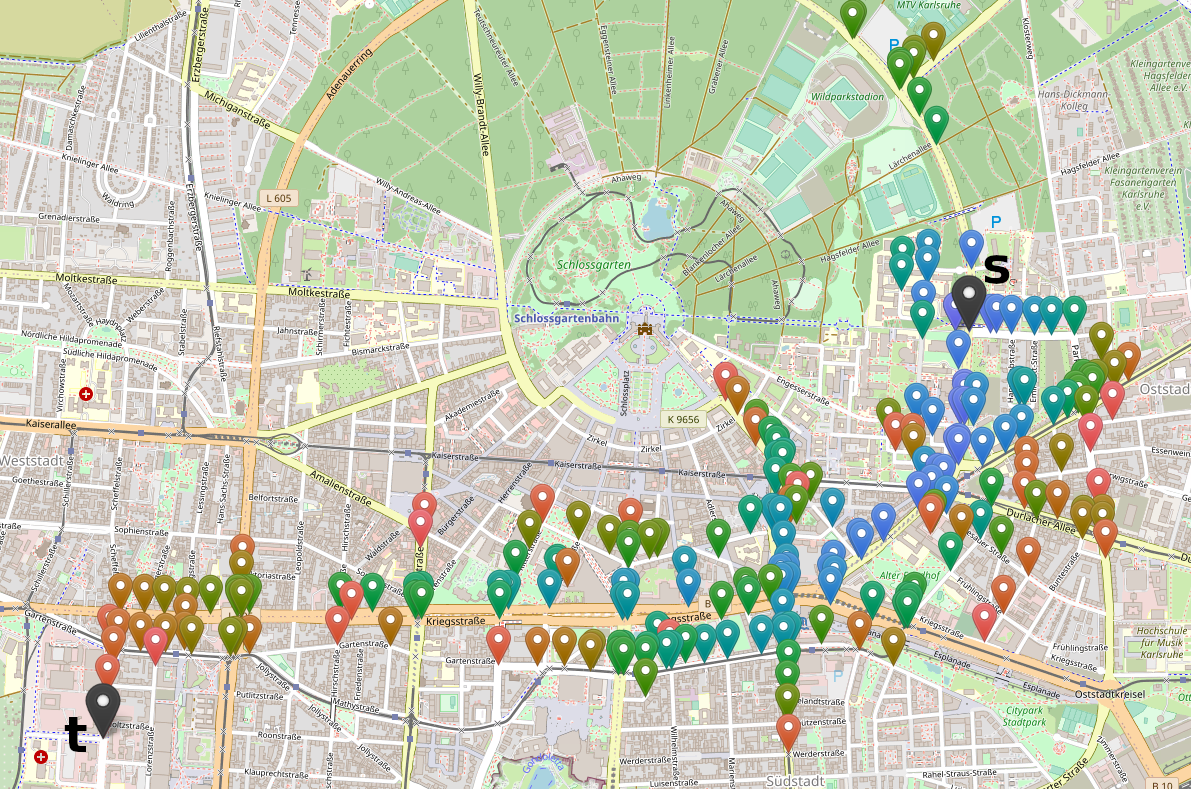
\includegraphics[width=.6\columnwidth]{fig/searchspace_st.png}
\caption{Vertices explored by A*. Color indicates the vertex removal order from the queue. Blue was removed first. Next is green. Red was removed last.}
\label{img:search-space}
\Description[A map where vertices visited by A* are marked.]{
A map of Karlsruhe where vertices visited by A* are marked.
The shape of the area with the visited vertices is similar to a drop.
The source vertex roughly lies in the center of the drop, the target vertex at the tip.
}
\end{figure}

\subsection{Contraction Hierarchies}

\begin{figure}
\centering
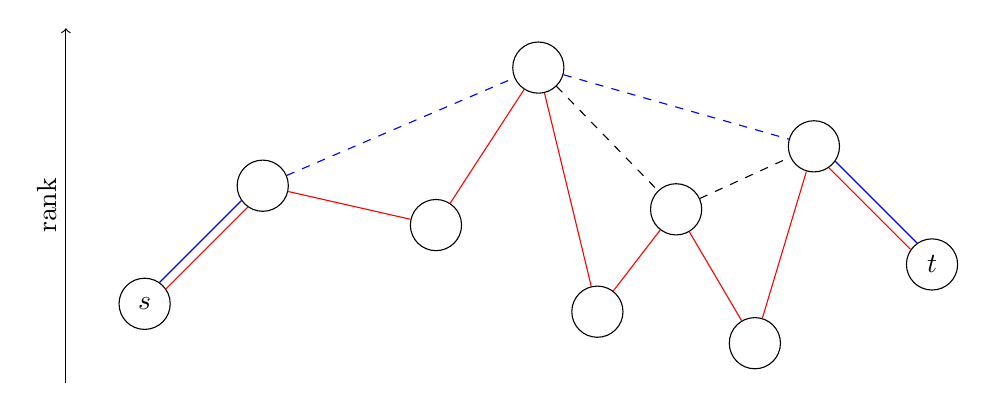
\begin{tikzpicture}[]
\tikzset{auto rotate/.style={to path={let \p1=(\tikztostart),\p2=(\tikztotarget),
\n1={atan2(\y2-\y1,\x2-\x1)},\n2={\n1-10},\n3={\n1+190}
in (\tikztostart.\n2) -- (\tikztotarget.\n3) \tikztonodes}}}

\node (s) at (0,0)     [node] {$s$};
\node (2) at (1.5,1.5) [node] {};
\node (3) at (3.7,1)   [node] {};
\node (4) at (5,3)     [node] {};
\node (5) at (5.75,-0.1)  [node] {};
\node (6) at (6.75,1.2)   [node] {};
\node (7) at (7.75,-0.5)    [node] {};
\node (8) at (8.5,2)   [node] {};
\node (t) at (10,0.5)  [node] {$t$};

\draw[->] (-1,-1) -- (-1,3.5) node [midway, above, sloped] { rank };

\draw (s) edge[red, auto rotate] (2);
\draw[red] (2) -- (3);
\draw[red] (3) -- (4);
\draw[red] (4) -- (5);
\draw[red] (5) -- (6);
\draw[red] (6) -- (7);
\draw[red] (7) -- (8);
\draw (8) edge[red, auto rotate] (t);

\draw (2) edge[blue, auto rotate] (s);
\draw[blue, dashed] (2) -- (4);
\draw[blue, dashed] (4) -- (8);
\draw (t) edge[blue, auto rotate] (8);

\draw[dashed] (4) -- (6);
\draw[dashed] (6) -- (8);
\end{tikzpicture}
\caption{
Solid lines are edges in $G$. Dotted lines are shortcuts. Red is a shortest $st$-path in $G$. Blue is equally long up-down $st$-path in $G^+$.
}
\label{fig:ch}
\Description[Vertices and edges of a shortest path in the original graph and the corresponding path in the augmented graph.]{
Vertices and edges of a shortest path in the original graph and the corresponding path in the augmented graph.
The y-position on the figure indicates the rank of each vertex.
Where the original shortest path down and then up, a shortcut edge connects the two higher vertices.
The path in the augmented graph goes only up and then down.
}
\end{figure}

\begin{algorithm2e}[tb]
\KwData{$D^{\downarrow}[v]$: tentative distance from any vertex $v \in V$ to target $t$ in $\gchd$}
\KwData{Minimum priority queue $Q$, ordered by tentative distances}
$D^{\downarrow}[v] \gets +\infty$ for all $v\neq t$\;
$D^{\downarrow}[t] \gets 0$\;
Make $Q$ only contain $t$ with tentative distance $0$\;
\While{$Q$ not empty}{
  $u\gets$ pop minimum element from $Q$\;
  \For{all reversed downward edges $uv \in \rechd$}{
    \If{$D^{\downarrow}[u] + \overleftarrow{w}(uv) < D^{\downarrow}[v]$}{
      $D^{\downarrow}[v] \gets D^{\downarrow}[u] + \overleftarrow{w}(uv)$\;
      Add $v$ or decrease $v$'s key in $Q$ to $D^{\downarrow}[v]$\;
    }
  }
}
\caption{CH backward search.}
\label{algo:ch-backward}
\end{algorithm2e}

\emph{Contraction Hierarchies} (CH) is a two-phase speedup technique to accelerate shortest path computations on road networks through precomputation.
For a detailed discussion we refer to~\cite{gssv-erlrn-12}.
Here, we only briefly introduce necessary notation and algorithms used in this paper.
In a preprocessing phase, vertices are ordered totally by ``importance'' where more important vertices should lie on more shortest paths.
Intuitively, vertices on highways are more important than vertices on rural streets.
For CH, such an ordering is obtained heuristically.
The position of a vertex in the order is also denoted as its \emph{rank}.
Vertices of higher rank are informally referred to and visualized as ``higher up'' in the hierarchy.
Therefore, an edge where the tail has lower rank than the head is an \emph{upward} edge.
Analogously, when the head vertex has the lower rank, the edge is said to go \emph{downward}.
Once such an importance ordering was obtained, all vertices are contracted successively by ascending importance.
To \emph{contract} a vertex means to temporarily remove it from the graph while inserting \emph{shortcut edges} between more important neighbors to preserve shortest distances among them.
The result is an \emph{augmented graph} $G^+$ with original edges and shortcuts.
We often refer to the augmented graph split into an upward graph $\gchu = (V, \echu)$ containing only upward edges and a downward graph $\gchd = (V, \echu)$ containing only downward edges.

The augmented graph has the property that for any two vertices $s$ and $t$, there always exists an \emph{up-down} $st$-path, i.e.\ a path  which first uses only edges from $\echu$ and then only edges from $\echd$, with the same length as a shortest path in $G$.
See Figure~\ref{fig:ch} for an illustration.
From every shortest path (red) in $G$, an up-down path of equal length in $G^+$ (blue) can be constructed.
Such an up-down path can be found by running Dijkstra's algorithm from $s$ on $\gchu$ and from $t$ on the reversed downward graph $\rgchd$ graph.
By construction, at least the highest ranked vertex on the up-down path must be in the intersection of the forward and backward search spaces.
Pseudocode for the backward search is presented in Algorithm~\ref{algo:ch-backward}.
The set of vertices reachable in $\gchu$ and $\rgchd$ is called the \emph{CH search space} of a vertex.
The CH query performance strongly correlates with the size of this CH search space and the number of edges between the vertices in the search space.
Luckily, on road networks, the CH search space is small~\cite{gssv-erlrn-12,dgpw-crprn-13}.

\subsection{Customizable Contraction Hierarchies}
\label{sec:cch-intro}

Customizable Contraction Hierarchies~\cite{dsw-cch-15} (CCH) is a variant of Contraction Hierarchies extended to a three-phase setup.
The phases consist of a slow preprocessing phase, a faster \emph{customization} phase, and the accelerated \emph{query} phase.
The preprocessing phase typically takes hours, the customization seconds, and the query fractions of a millisecond.
The preprocessing phase is independent of the weights and only uses the graph topology.
Weights are introduced in the customization phase.
Shortest paths are computed in the query phase.

The key idea for CCH is to use a vertex importance order that is independent of the weight function.
CCH use \emph{nested dissection} orders for this.
A small balanced vertex separator is computed and the separator vertices get the highest importance.
The remaining vertices are ordered by recursing on the independent cells obtained by removing the separator vertices.
This results in surprisingly good CH orders.
Regardless of the weight function, any shortest path between the cells has to use some of the separator vertices, therefore these vertices will always be ``important''.
Such orders can be obtained with partitioning algorithms tailored to road networks~\cite{GottesburenHUW19} in less than an hour even for continental-sized road networks.
Once the order was computed, the augmented graph $G^+$ is computed.
The standard CH preprocessing algorithms could be used for this but specialized, significantly faster CCH variants exist.
However, discussing them in detail is beyond the scope of this work.
See~\cite{dsw-cch-15,DBLP:journals/jea/Buchhold0W19} for details.
A CCH augmented graph fulfills all necessary properties for CH query algorithms.
The CH query algorithms can therefore be applied without modifications.
However, the CCH preprocessing grants some useful additional properties.

During preprocessing, an \emph{elimination tree} can be constructed.
The root of the elimination tree is the most important vertex.
For every other vertex, its parent is its least important upward neighbor.
In~\cite{bcrw-s-16}, it was proven that the set of ancestors of a vertex in the elimination tree is equal to its CH search space.
This makes it possible to explore the CCH search space with a more efficient shortest path algorithm:
For the forward search, start at the source and follow the elimination tree upward until the root is reached.
All outgoing edges of encountered vertices are relaxed.
The backward search works analogously but starts at the target.
Because this elimination tree-based algorithm does not require a queue, it is faster than a Dijkstra-based CCH query.
With this algorithm, CCH can consistently answer shortest path queries on continental sized road networks in fractions of a millisecond.
CH queries are still marginally faster for weight functions with a strong hierarchy such as travel times.
However, on weight functions with a less pronounced hierarchy, CH performance degrades significantly and CCH queries turn out the faster variant.
Note that only nested dissection orderings admit an elimination tree of low height.
Thus, the elimination tree query can not be used with classical CH.

\subsection{PHAST}

\begin{algorithm2e}[tb]
\KwData{$D[v]$: tentative distance from any $v \in V$ to $t$}
Execute Algorithm~\ref{algo:ch-backward}, filling $D$\;
\For{all CH levels $L$ from most to least important}{
	\For{all up-edges $uv \in \echu$ with $u$ in $L$}{
		\If{$D[u] > D[v] + w(uv)$}{
			$D[u] \leftarrow D[v] + w(uv)$\;
		}
	}
}
\caption{PHAST basic all-to-one search.}
\label{algo:phast}
\end{algorithm2e}

PHAST~\cite{dgnw-phast-13} is a CH extension that computes distances from all vertices to one target vertex (or vice versa, the reverse case works analogously).
This is sometimes denoted as a \emph{all-to-one} (or \emph{one-to-all}) problem.
The preprocessing phase remains the same as for CH.
The query phase is split into two steps.
The first step is analogue to the CH query:
From $t$, all reachable vertices via reversed down-edges are explored as shown in Algorithm~\ref{algo:ch-backward}.
For the second step, PHAST utilizes an assignment of vertices into \emph{levels}.
These levels correspond to the importance ordering but allow multiple vertices in the same level.
However, no edge must connect two vertices within the same level.
Such a level assignment can be obtained by assigning all vertices without lower-ranked neighbors to the lowest level.
All other vertices are then iteratively assigned to the next level above the highest level of any downward neighbor.

The main work of the second step consists in iterating over all CH levels from top to bottom.
In each iteration, all up-edges starting within the current level are relaxed in reverse.
After all levels are processed, the shortest distances from all vertices to $t$ were computed.
Pseudocode is provided in Algorithm~\ref{algo:phast}.
PHAST is faster than Dijkstra's algorithm on road graphs because it is a better fit for modern processor architectures, better at utilizing data locality and, most importantly, can be parallelized very effectively.
% However, we will not consider parallelization in this paper.
See~\cite{dgnw-phast-13} for an in-depth experimental performance analysis.
% Using PHAST, we can also compute a tight A* heuristic.
% In the query phase, we first run PHAST to compute the distances from every vertex to $t$ with respect to $w$ and store the result in an array $H$.
% Next, we run $A^*$ and implement the heuristic as a lookup in the array $H$.

% This PHAST-based algorithm works.
% The $H$ lookup and by extension the $A^*$ search is indeed fast.
% However, the PHAST step before the search is comparatively expensive.
% The reason is that the distances towards $t$ are computed for \emph{all} vertices.
% Ideally, we only want to compute the distances from the vertices explored in the $A^*$ search.

\subsection{RPHAST}

RPHAST~\cite{delling_et_al:OASIcs:2011:3266}, short for Restricted PHAST, is a PHAST extension for efficiently computing distances from a smaller set of source vertices to one target vertex (again, the reverse case works analogously), solving the \emph{many-to-one} problem.
Given a set of source vertices $S$, the first step is to copy the combined search space of all sources into a \emph{restricted subgraph}.
Let $V_{\operatorname{restr}}$ be the set of vertices reachable in $\gchu$ from any $s_i \in S$.
The restricted subgraph $\gchu_{\operatorname{restr}}$ is subgraph of $\gchu$ induced by $V_{\operatorname{rest}}$.
Finding and copying the relevant edges into this restricted subgraph makes up the \emph{selection} step.
In the query step, a target $t$ is given and the PHAST algorithm is applied but the downward sweep (second step of the PHAST algorithm) is performed only on the restricted subgraph.
RPHAST is particularly effective when many targets are queried for the same source set $S$.
If the source set changes often, selection times may become problematic.
% RPHAST can also be applied to the \emph{many-to-many} problem, computing a distance matrix between sets $S$ and $T$ of vertices.
% Implemented with SIMD instructions it is, to the best of our knowledge, the fastest currently known algorithm for this problem setting.

\section{The Incremental Many-to-One Problem}\label{sec:lazy-rphast}

In this section, we discuss a variant of the many-to-one shortest path problem which naturally arises from A* heuristics.
Here, the target vertex $t$ is known in the selection step, but source vertices $s_1,\dots,s_k$ are queried one after another.
We denote this problem as the \emph{incremental many-to-one} problem.
The first step is the \emph{target selection} where the target vertex $t$ is provided.
Then, an arbitrary number of source vertices are given one after another.
For each source $s_i$ the distance $\dist(s_i, t)$ has to be computed before the next source $s_{i+1}$ is provided.

We consider the combined running time of the target selection and each incremental query as the total running time to answer an incremental many-to-one query.
Since the target selection time is included, computing the distances to all vertices with Dijkstra or PHAST is too slow.
Also, since the source set is provided incrementally, RPHAST in its basic form is not well suited to our problem.
Fortunately, we can do better.

\subsection{Lazy RPHAST on Contraction Hierarchies}

\begin{algorithm2e}[tb]
\KwData{$D^{\downarrow}[v]$: tentative distance from any vertex $v \in V$ to $t$ as computed by Algorithm~\ref{algo:ch-backward}}
\KwData{$D[v]$: memoized distance from vertex $v \in V$ to $t$, shared between invocations, initialized to $\bot$ during the selection}
\SetKwFunction{Dist}{ComputeAndMemoizeDist}
\SetKwProg{Fn}{Function}{:}{}

Execute Algorithm~\ref{algo:ch-backward}, filling $D^{\downarrow}$\;
$D[v] \gets \bot$ for all $v \in V$\;

\Fn{\Dist{$u$}}{
	\If{$D[u] = \bot$}{
		$D[u]\leftarrow D^{\downarrow}[u]$\;
		\For{all up-edges $uv \in \echu$}{
      $D[u]\leftarrow\min(D[u],w(uv)+\Dist(v))$\;
		}
	}
	\Return{$D[u]$}\;
}
\caption{Lazy RPHAST algorithm.}
\label{algo:lazy_rphast_ch}
\end{algorithm2e}

The core idea of our algorithm is to do the RPHAST computation lazily and using memoization.
In the target selection, we first run the backward CH search from $t$ to obtain an array $D^{\downarrow}$.
$D^{\downarrow}[v]$ is the minimum down $vt$-path distance or $+\infty$, if there is no such path.
$D^{\downarrow}$ is computed as shown in Algorithm~\ref{algo:ch-backward}.
Further, the distances $D[v]$ are initialized to a sentinel value $\bot$ where $\bot$ is some special value distinct from any other valid distance (including $\infty$).
This value indicates that the distance to from $v$ to $t$ has not yet been computed.

Now, distances from many sources $s_i$ to $t$ can be computed incrementally with the \textsf{ComputeAndMemoizeDist} function as shown in Algorithm~\ref{algo:lazy_rphast_ch}.
The key to doing this efficiently is reusing the distance information $D$ across invocations through memoization.
Thus, the first step of the algorithm is always to check if the distance for the requested vertex has already been computed and immediately returning it if this is the case.
If not, the distance $D[s_i]$ is initialized to the shortest down-path distance $D^{\downarrow}[s_i]$ obtained by the backward search.
Then, the algorithm iterates over all up-edges $(s_i v)$ and checks if the up-down path through this neighbor can improve the distance.
To obtain the shortest distance from a neighbor $v$ to $t$, the algorithm is invoked recursively.

\paragraph{Correctness}
Due to~\cite{gssv-erlrn-12}, an up-down path of shortest distance must exist in $G^+$.
Further, $G^+$ can be decomposed into two directed acyclic graphs (DAG) $\gchu$ and $\gchd$ and the up path can be found in $\gchu$ and the down path in $\gchd$.
Observe that the second part of Lazy RPHAST is, in fact, a recursive depth-first search (DFS) on $\gchu$ which relaxes edges $uv$ in reverse topological order of the tail vertices $u$.
Since DFS can be used to find shortest paths on DAGs, the search will find shortest up paths on $\gchu$.
Concatenated with the down paths obtained by the backward search, this yields correct shortest distances.

\subsection{Lazy RPHAST on Customizable Contraction Hierarchies}

Algorithm~\ref{algo:lazy_rphast_ch} can be applied to CCH without any modifications.
However, we can also exploit the elimination tree in the Lazy RPHAST algorithm.
To compute the distance $D[v]$ of a vertex $v$, the distances of all upward neighbors must be final.
In Algorithm~\ref{algo:lazy_rphast_ch}, these upward neighbor distances are computed recursively.
Thus, the search space is explored in a DFS-like fashion and distances are finalized in DFS post order.
However, the path from a vertex to the root in the elimination tree is a also topological order for the upward search space.
This is because the ancestors in the elimination tree contain the entire upward search space~\cite{bcrw-s-16}.
Therefore, iterating over the vertices on the elimination tree path from the root to $v$ while relaxing outgoing upward edges of each vertex also yields shortest distances.
Further, with this approach, when a vertex $v$ already has a distance $D[v] \neq \bot$, all ancestors of $v$ must already have their final distance, too.
Thus, as soon as the algorithm encounters a vertex which already has a final distance, the remaining search space is known to have final distances.

\begin{algorithm2e}[tb]
\KwData{$D^{\downarrow}[v]$: tentative distance from any vertex $v \in V$ to $t$ as computed by Algorithm~\ref{algo:ch-backward}}
\KwData{$D[v]$: memoized distance from any vertex $v \in V$ to $t$, shared between invocations, initialized to $\bot$ during the selection}
\KwData{$P[v]$: parent of a vertex $v \in V$ in the elimination tree, a parent of $\bot$ indicates the root vertex}
\KwData{$S$: stack with vertices to compute distances, empty initially, only used to store intermediate data}
\SetKwFunction{Dist}{ComputeAndMemoizeDist}
\SetKw{Break}{break}
\SetKwProg{Fn}{Function}{:}{}

Execute Algorithm~\ref{algo:ch-backward}, filling $D^{\downarrow}$\;
$D[v] \gets \bot$ for all $v \in V$\;

\Fn{\Dist{$u$}}{
  \tcp{Determine the vertices $v$ for which $D[v]$ needs to be computed}
  $v \gets u$\;
	\While{$D[v] = \bot$}{
    Push $v$ onto $S$\;
		\If{$P[v] = \bot$}{
      \Break\;
		}
    $v \gets P[v]$\;
  }
  \tcp{Compute $D$ for those vertices}
  \While{$S$ not empty}{
    $v\leftarrow$ pop top element from $S$\;
		$D[v]\gets D^{\downarrow}[v]$\;
		\For{all up-edges $vw \in \echu$}{
      $D[v]\gets\min(D[v],w(vw)+D[w])$\;
		}
	}
	\Return{$D[u]$}\;
}
\caption{Elimination tree based Lazy RPHAST algorithm.}
\label{algo:cch_pot}
\end{algorithm2e}

This allows for the more efficient implementation depicted in Algorithm~\ref{algo:cch_pot}.
For any vertex which already has a memoized distance $D[v] \neq \bot$, the algorithm immediately returns this distance.
To compute missing distances, the elimination tree ancestors which also do not have a distance yet are collected onto a stack $S$.
The elimination tree can be traversed through parent pointers $P[v]$.
As soon as a vertex with final distance is encountered, all remaining ancestors are known to have their final distance.
Now, the vertices are successively popped from the stack, i.e.\ the algorithm walks the elimination tree path back down and relaxes outgoing upward edges.
This yields the shortest distances for all the vertices on the path.

% \subsection{Many-to-Many with Lazy RPHAST}

% RPHAST was originally developed to answer many-to-many queries.
% It was not designed to be used in conjunction with A*.
% Investigating how Lazy RPHAST performs in the many-to-many setting is therefore interesting.
% In this setting, a set of source and target vertices are given.
% The objective is to compute the distances between all pairs of source and target vertices.
% In this section, we described how Lazy RPHAST can be used to solve this many-to-many problem.
% Our experiments will show, that the achieved performance is comparable to the original RPHAST algorithm.

% To solve the many-to-many problem, RPHAST uses SIMD vector instructions.
% Let $k$ denote the number of elements in one vector.
% RPHAST computes the distances from all source vertices to $k$ target vertices in one run.
% If the target set contains more than $k$ vertices, then the target set is split into smaller sets of $k$ elements\footnote{If the number of targets is not divisible by $k$, the set is increased by adding additional target vertices.}.
% The algorithm is then run for each of these smaller sets.
% Each RPHAST run performs vectorized variants of the selection and query phases.\todo{Is query phase definiert?}

% We translate this setup to the Lazy RPHAST setting as follows.
% First, a set of $k$ target vertices need to be fixed.
% A vectorized selection phase is then performed for this fixed target set.
% After the selection, the source vertices are iteratively revealed.
% Once a source vertex is revealed, the algorithm must compute the distances to all $k$ targets.
% Only after the distances are computed, the next source vertex is revealed.

% The core of Lazy RPHAST are the Algorithms~\ref{algo:ch-backward} and~\ref{algo:lazy_rphast_ch}.
% We describe vectorized variants of these algorithms.
% We replace the $B$ and $D$ arrays of scalars by arrays of $k$-dimensional vectors of scalars.
% To clarify which entities are SIMD vectors, we denote the vectorized arrays by $\hat{B}$ and $\hat{D}$.
% $\hat{D}[s]$ is an SIMD vector $\hat{v}$ of length $k$.
% The $i$-th element $\hat{v}[i]$ of $\hat{v}$ will contain the distance from $s$ to $i$-th selected target.
% We can also denote this distance using $\hat{D}[s][i]$.
% All operations on SIMD vectors are component-wise.
% Adding a scalar to an SIMD vector consists of adding the scalar to every element of the SIMD vector.

% \todo{Rechtschreibung: down edge vs down-edge und up edge vs up-edge. Geht beides aber bitte konsistent.}

% \begin{algorithm2e}
% \KwIn{$\hat{T}$: SIMD vector of $k$ target vertices}
% \KwData{$\hat{B}[x][i]$: tentative distance from $x$ to target $\hat{T}[i]$}
% \KwData{Minimum priority queue $Q$, also called open list, ordered by vertex rank}
% Make $Q$ an empty queue\;
% $\hat{B}[x][i] \leftarrow +\infty$ for all $x$ and $i$\;
% \For{all $i\in \{0\ldots k-1\}$}{
%   $\hat{B}[\hat{T}[i]][i] \leftarrow 0$\;
%   Add $\hat{T}[i]$ to $Q$\;
% }
% \While{not $Q$ empty}{
%   $y\leftarrow$ pop minimum element from $Q$\;
%   \For{all down-edges $xy$  in $G^+_\ell$}{
%     $\hat{B}[x] \leftarrow \min\{\hat{B}[x], \hat{B}[y] + w_\ell(xy)\}$\;
%     Add $x$ to $Q$ if not in $Q$\;
%   }
% }
% \caption{Vectorized Lazy RPHAST selection}
% \label{algo:simd-ch-backward}
% \end{algorithm2e}

% Vectorizing Algorithm~\ref{algo:ch-backward} needs some adjustments.
% In the original algorithm, the vertices are ordered by distance.
% In the vectorized variant, distances are SIMD vectors and can therefore not be ordered.
% To resolve this problem, we ordered the vertices in the queue not by distance but by CH rank.
% The CH rank is the position of a vertex in the contraction order. \todo{wurde rank schon eingeführt? Falls ja, dann kann der Satz weg.}
% All other modifications are straightforward.
% The vectorized version is presented in Algorithm~\ref{algo:simd-ch-backward}.
% Algorithm~\ref{algo:lazy_rphast_ch} can be vectorized by just replacing the arrays by their SIMD variants.
% The result is illustrated in Algorithm~\ref{algo:simd-pot}.


% \begin{algorithm2e}
% \KwData{$\hat{B}[x][i]$: tentative distance from $x$ to $\hat{T}[i]$ as computed by Algorithm~\ref{algo:simd-ch-backward}}
% \KwData{$\hat{D}[x][i]$: memoized distance from $x$ to $\hat{T}[i]$, $\bot$ initially}
% \SetKwFunction{VecDist}{SIMDComputeAndMemoizeDist}
% \SetKwProg{Fn}{Function}{:}{}
% \Fn{\VecDist{$x$}}{
%   \If{$\hat{D}[x] = \bot$}{
%     $\hat{D}[x]\leftarrow \hat{B}[x]$\;
%     \For{all up-edges $xy$ in $G^+_\ell$}{
%       $\hat{D}[x]\leftarrow\min\{\hat{D}[x],w_\ell(xy)+\VecDist(y)\}$\;
%     }
%   }
%   \Return{$\hat{D}[x]$}\;
% }
% \caption{Vectorized Lazy RPHAST algorithm}
% \label{algo:simd-pot}
% \end{algorithm2e}


% \todo{Hier beginnt der ältere Text}
% Since SSE RPHAST is the fastest known algorithm for many-to-many computations, investigating the Lazy RPHAST performance in this setting seems worthwhile.
% SSE RPHAST starts by performing the selection phase on the full target set.
% % TODO flip directions?
% Second, a query is performed for each source which yields the distances from this source to all targets (RPHAST).
% This second step can be improved by processing $k$ (typically 16) sources at once using SIMD vector instructions (SSE RPHAST).
% Naively translating this approach to Lazy RPHAST would mean selecting one target after another and for each doing the full lazy exploration from all sources.
% However, this approach would explore the upward search space of all the sources multiple times.
% This work seems redundant.

% Luckily, we can do better by integrating a different One-to-Many CH variant -- the Bucket-CH algorithm~\cite{gssv-erlrn-12} -- to select all targets at once.
% The Bucket CH selection phase works as follows:
% % TODO better structure or local outline
% % TODO besser herleiten, wieso kein 2d array
% For each vertex $x$, we maintain an initially empty list $B[x]$ of pair $(t_i, \textrm{dist}_{\textrm{up}}(x,t_i))$.
% These pairs are called \emph{buckets}.
% These buckets are populated by running a backward CH search (Algorithm~\ref{algo:ch-backward}) from each $t_i$ and inserting the resulting distances into the buckets.
% Now Algorithm~\ref{algo:lazy_rphast_ch} (or~ Algorithm~\ref{algo:cch_pot}) can compute distances from a given source to \emph{all} targets at once.
% We only have to change $D[x]$ so that it is an array of distances to each $t_i$ instead of a single scalar value.
% After calling the adjusted \texttt{ComputeAndMemoizeDist} for each source, we know the shortest distances between each pair of source and target vertex.
% This way, the search space of the sources is explored only once.

% The Bucket-CH selection phase still explores the shared parts of the search space of the targets several times.
% This can be improved with the following modified CH backward search:
% All target vertices are inserted into the queue at once.
% The priority queue is ordered by importance instead of distance.
% Distance labels are buckets instead of scalar values.
% The buckets of each target vertex are initialized with a single entry for the respective vertex with distance zero.
% When relaxing an edge, the entries in the current vertex's bucket are increased by the edge's weight and merged with the bucket entries of the head vertex of the edge.
% By keeping the buckets sorted, this merging can be efficiently implemented with a coordinated linear sweep over both buckets.
% We evaluate our Lazy RPHAST many-to-many algorithm with this improved Bucket-CH selection in Section~\ref{sec:exp_lazy_rphast}.
% % TODO describe improved^2 Bucket CH

\section{Optimizations for A* in Road Networks}\label{sec:astar_opts}

In this section, we propose optimizations for A* in road networks.
First, we present several low degree vertex optimizations which exploit road network characteristics to reduce the overhead of queue operations and heuristic evaluations.
Second, we discuss the bidirectional A* algorithm and propose an improved pruning criterion for symmetric bidirectional potentials.
These optimizations can be used with \emph{any} A* heuristic.

\subsection{Low Degree A* Improvements}\label{sec:low-deg-improvment}

Preliminary experiments showed that a significant amount of query running time is spent in heuristic evaluations and queue operations.
We can reduce both by keeping some vertices out of the queue, as the heuristic needs to be evaluated when a vertex is pushed into the queue.
Consider for example a chain of vertices with exactly two neighbors.
Traversing this chain by successively pushing each vertex into the queue, computing the heuristic and popping the vertex again from the queue appears quite wasteful.
Therefore, we now discuss techniques to process such vertices consecutively without the queue.
The techniques discussed here are essentially a lazy variant of the ideas used in TopoCore~\cite{DBLP:conf/gis/DibbeltSW15}.

% We modify A* by processing low degree vertices consecutively without pushing them into the queue.
% Analogously to A*, our algorithm stores for every vertex $v$ a tentative distance $D[v]$ and maintains a minimum priority queue.
% Diverging from A*, not all vertices need be pushed into the priority queue even though every vertex has a tentative distance.

\subsubsection{Skip Degree Two Vertices}

Recall that $|N(u)|$ is the number of neighbors $v$ such that $vu \in E$ or $uv \in E$.
Our algorithm differs from classical A* when removing a vertex $u$ from the queue.
A* iterates over the outgoing edges $uv$ of $u$ and tries to reduce $D[v]$ by relaxing $uv$.
If A* succeeds, $v$'s weight in the queue is set to $D[v]+h_t(v)$.
Our algorithm, however, behaves differently, if $|N(v)|\le 2$.
Our algorithm determines the longest degree two chain of vertices $u, v_1,\ldots, v_k, w$ such that $|N(v_i)|=2$ and $|N(w)| > 2$.
If our algorithm succeeds in reducing $D[v_1]$, it does not push $v_1$ into the queue.
Instead, it iteratively tries to reduce all $D[v_i]$.
If it does not reach $w$, then only $D$ is modified, but no queue action is performed.
If $D[w]$ is modified and $|N(w)|>2$, $w$'s weight in the queue is set to $D[w]+h_t(w)$.

As the target vertex $t$ might have degree two, our algorithm cannot rely on stopping when $t$ is removed from the queue.
Instead, our algorithm stops as soon as $D[t]$ is less than the minimum weight in the queue.

\subsubsection{Skip Degree Three Vertices}

We can also skip some degree three vertices.
Denote by $u, v_1,\ldots, v_k, w$ a degree two chain as described in the previous section.
If $|N(w)| > 3$ or $w$ is in the queue, our algorithm proceeds as in the previous section.
Otherwise, there exist up to two degree chains $w, x_1,\ldots,x_p, y$ and $w,a_1,\ldots,a_q,b$ such that $x_1\neq v_k \neq a_1$.
Our algorithm iteratively tries to reduce all $D[x_i]$ and $D[a_i]$.
If it reaches $b$, $b$'s weight in the queue is set to $D[b]+h_t(b)$.
Analogously, if $y$ is reached, $y$'s weight is set to $D[y]+h_t(y)$.
If neither $y$ nor $b$ are not reached, no queue operation is performed.

\subsubsection{Stay in Largest Biconnected Component}\label{sec:largested-biconnected-component}

A lot of vertices in road networks lead to dead-ends.
Unless the source or target is in this dead-end, it is unnecessary to explore these vertices.

In the preprocessing phase, we compute the subgraph $G_C$, called \emph{core}.
$G_C$ is induced by the largest biconnected component of the undirected graph underlying $G$.
We do this using Tarjan's algorithm \cite{t-dfslg2-72}.
For every vertex $v$ in the input graph $G$, we store the attachment vertex $a_v$ to the core.
For vertices in the core, $a_v=v$.
We exploit that all attachment vertices are single vertex separators and the problem can be decomposed along them.

The query phase is divided into two steps.
In the first step, we apply A* to $G_C$ combined with the component that contains $s$.
This can be achieved implicitly by removing edges from $G_C$ into other components.
If $t$ is part of $G_C$ or in the same component as $s$, this A* search finds it.
Otherwise, we find $a_t$.
In that case, we continue by searching a path from $a_t$ towards $t$ restricted to $t$'s biconnected component.
The final result is the concatenation of both paths.

\subsection{Bidirectional A*}\label{sec:bidir_astar}

On road graphs, bidirectional search provides a simple way to halve the practical running time of Dijkstra's algorithm.
A bidirectional variant of A* therefore also seems desirable.
However, as shown in~\cite{gh-cspas-05}, the necessary modifications are not straightforward.
We revisit bidirectional A* and propose an alternative approach.
Our experiments show that it is competitive with the solution described by~\cite{gh-cspas-05}.

The straightforward idea is to use two heuristics $\overrightarrow{h}_t(v)$ and $\overleftarrow{h}_s(v)$.
The forward search has its queue ordered by $\overrightarrow{D}[v] + \overrightarrow{h}_t(v)$, where $\overrightarrow{h}_t(v)$ estimates the distance $\dist(v,t)$ from $v$ to $t$.
Similarly, the backward search has its queue ordered by $\overleftarrow{D}[v] + \overleftarrow{h}_s(v)$, where $\overleftarrow{h}_s(v)$ is an estimate of the distance $\dist(s,v)$ from $s$ to $v$.
% We denote by $\overrightarrow{k}$ and $\overleftarrow{k}$ the minimum queue keys and by $\mu$ the length of the shortest $st$-path found so far.

The problem with this straightforward approach is that these two potentials induce different reduced graphs (see Section~\ref{sec:a_star}).
Thus, in the equivalent bidirectional Dijkstra search each direction would run on a different graph.
This breaks the usual bidirectional Dijkstra stopping criterion.
To the best of our knowledge, no better stopping criterion exists than running \emph{both} searches until the unidirectional stopping criterion is met for either direction.
The forward search can skip vertices already settled by the backward search and vice versa.
However, this straightforward bidirectional A* still performs more work than a unidirectional A*~\cite{gh-cspas-05}.
Thus, on its own it is not a useful algorithm.
However, it can serve as basis for further algorithmic refinements.
The authors of~\cite{gh-cspas-05} refer to this as \emph{symmetric} bidirectional A*.

To obtain a bidirectional stopping criterion, the \emph{average potential} is proposed~\cite{gh-cspas-05}.
It combines a forward and a backward heuristic $\overrightarrow{h}_t$ and $\overleftarrow{h}_s$ into a combined \emph{average heuristic} $h_{\overline{st}}$.
The idea is to use a common reduced graph, whose weights are the average weights of the individual reduced graphs.
Both searches run on the same common reduced graph.
This allows stopping the searches when $\overrightarrow{k} + \overleftarrow{k} \geq \mu$.
Formally, $h_{\overline{st}}(v)$ is defined as $(\overrightarrow{h}_t(v) - \overleftarrow{h}_s(v))/2$.
The forward search uses $h_{\overline{st}}(v)$ as its heuristic.
The backward search uses $-h_{\overline{st}}(v)$.
Unfortunately, average potentials have two downsides.
First, evaluating the average potential requires evaluating both $\overrightarrow{h}_t$ and $\overleftarrow{h}_s$.
Evaluating the average heuristic is therefore slower than evaluating just one of the composing heuristics.
Second, the bidirectional stopping criterion comes at the cost of worse estimates for each direction on its own.
$h_{\overline{st}}(v)$ is a worse estimate for $\dist(v,t)$ than $\overrightarrow{h}_t$.
Similarly, $-h_{\overline{st}}(v)$ is a worse estimate for $\dist(s,v)$ than $\overleftarrow{h}_s$.\footnote{
To obtain an actual lower bound from this average heuristic, one has to add $\overleftarrow{h}_s(t)/2$ in the forward case and $\overrightarrow{h}_t(s)/2$ in the backward.
Adding any constant to a heuristic function does not change the reduced graph.
}
The second downside can be partially mitigated through pruning with the composing heuristics.
When the forward search scans an edge $uv$ where $\overrightarrow{D}[u] + w(uv) + \overrightarrow{h}_s(v) > \mu$ holds, i.e. the distance plus the estimate of the remaining distance is already greater than the currently known tentative distance, it is not necessary to push $v$ into the queue.
The pruning rule for the backward search is analogous.

To avoid the downsides of the average potential, we revisit symmetric bidirectional A* and propose a new pruning criterion.
We describe the idea for the forward search.
The pruning rule for the backward search is analogous.
The central idea consists of using information from the backward search to prune edges in the forward search.
We do not use the average heuristic.
Instead of a strong stopping criterion, we use a pruning rule that gets stronger the longer the search runs.
Such a pruning rule will eventually prune all remaining branches and stop the search.
The stopping criteria for each direction remain the same (unidirectional) as before.
However, usually the search stops early because the queues are empty.

Let $uv$ be an edge that we relax in the forward search.
Before pushing $v$ into the queue, we apply the new pruning rule.
If we can prove that every path using $uv$ is at least as long as the shortest known path length $\mu$, then we do not have to push $v$.
We therefore want to obtain a lower bound for $\dist(s,u)+w(uv)+\dist(v,t)$.
As $u$ was settled, $\overrightarrow{D}[u]$ contains the shortest path length $\dist(s,u)$, i.e., $\dist(s,u)=\overrightarrow{D}[u]$.
$w(uv)$ is also exactly known as it's just an edge weight.
It remains to lower bound $\dist(v,t)$.
Vertices are removed from the backward queue ordered by $\overleftarrow{h}(v) + \dist(v,t)$.
If $v$ was not yet removed from the backward queue, we know that $\overleftarrow{h}(v) + \dist(v,t) \geq \overleftarrow{k}$.
This gives us the required lower bound, i.e. $\dist(v,t) \geq \overleftarrow{k}-\overleftarrow{h}(v)$.
Thus, $v$ does not have to be pushed if $\overrightarrow{D}[u]+w(uv)+\overleftarrow{k}-\overleftarrow{h}(v)\ge \mu$.
The vertex $v$ might still be pushed into the queue when there is another edge $wv$ for which the pruning is not possible.
Checking the pruning rule requires evaluating the backward heuristic.
However, pruning is only possible once the searches have met, i.e. $\mu < \infty$.
Before that, each direction only has to evaluate its own heuristic.
Thus, our pruning improves on both downsides of the average potential.

Unless stated differently, for all bidirectional A* variants, we always alternate between removing a vertex from the forward and the backward queues.
In our experiments, we also evaluate expanding the search with the smaller minimum queue key.
While this may sound sensible, our experiments show in Table~\ref{tab:bidir_switching} that it is never beneficial in terms of running time.

\section{The CH-Potentials Framework}\label{sec:framework}

% , we describe how to use the Lazy RPHAST algorithm to build a fast and tight heuristic for A*.
In this section, we introduce an algorithmic framework to apply A* with a Lazy RPHAST-based heuristic to a variety of practical route planning problems.
We call our approach \emph{CH-Potentials}.
The core idea is to compute a CH augmented graph during preprocessing and use A* with a straightforward application of Lazy RPHAST as the heuristic to answer queries.
When the CH preprocessing and the A* algorithm are performed on the same graph with the same weight function, this yields a \emph{perfect} heuristic.
However, this case is, of course, not particularly interesting.
One could just answer the shortest path query directly with a CH query.
The approach becomes useful when the query runs on a \emph{different but related} graph or weight function than the preprocessing.
Therefore, we start by establishing a common formal framework for the use of CH-Potentials.
Then, we exemplarily describe some extended routing problems and how to apply the CH-Potentials framework to them.

\subsection{Formal Problem Setup: Inputs, Outputs, and Phases}\label{sec:formal_framework}

We consider a variety of different of applications, with slightly different problem models.
The goal is always to quickly answer many shortest path queries.
For the purpose of describing our framework, we establish a shared notation:
Input to each query are vertices $s$ and $t$, and a graph $G_q$ with query weights $w_q$.
However, the precise formal inputs of the query and what exactly $w_q$ represents depends on the application.
In the simplest case, $w_q$ will be scalar edge weights.
Live traffic is an example for this.
The challenge in this scenario is that values of $w_q$ might change between queries.
However, $w_q$ can also represent something more complex than scalar numbers.
It can be any function that computes a weight for an edge.
This function can also take additional parameters from the state of the search.
In the case of traffic predictions, $w_q$ is a function which maps the edge entry time to the traversal time and the query takes an additional departure time parameter.

To enable quick shortest path computations, we consider a two-phase setup with an additional offline preprocessing phase before the online query phase.
The input to the preprocessing phase is a lower bound graph $G_\ell = (V_{\ell}, E_{\ell})$ with lower bound weights $w_\ell$ where $w_\ell(e)$ must be a scalar value for every edge $e$ of $G_\ell$.
The output of the preprocessing is auxiliary data that allows to quickly compute distances on $G_\ell$ with respect to $w_\ell$.
In the applications considered in this paper, $w_\ell$ is always the \emph{free-flow} travel time.

The query phase may use this auxiliary data to answer shortest path queries between vertices $s$ and $t$ on $G_q = (V_q, E_q)$ with weights $w_q$.
Let $\phi : V_q \to V_{\ell}$ denote a function mapping vertices in the query graph to vertices in the lower bound graph.
The only requirement for a routing problem to fit into our problem framework is that the query weight of an edge $w_q(u v)$ is greater or equal to the shortest distance $\dist_\ell(\phi(u), \phi(v))$ between the corresponding vertices $\phi(u)$ and $\phi(v)$ in the lower bound graph $G_\ell$ with respect to $w_\ell$.
Unless stated otherwise, $G_q$ and $G_\ell$ are the same graph, $\phi$ is the identity function, and only $w_q$ changes for the queries.

\subsection{CH-Potentials}\label{sec:chpot}
CH-Potentials can be used to solve any problem in this setup.
The preprocessing is always the computation of the CH augmented graph $G^+_{\ell}$ and remains the same regardless of the specific routing problem.
The query consists of A* with the heuristic function $h_t(v) = \dist_{w_{\ell}}(\phi(v), \phi(t))$ computed using Lazy RPHAST.
In the beginning of each query, we perform the target selection, i.e.\ a backward CH search, from the target $t$.
The heuristic function $h_t(v)$ is implemented by a call to the \texttt{ComputeAndMemoizeDist} for vertex $\phi(v)$ (see Algorithm~\ref{algo:lazy_rphast_ch}).
Note that, in contrast to the preprocessing, the exact implementation of the A* search depends on the application.
Our approach only provides the heuristic $h_t$ for the A* search.
As the performance of A* depends crucially on the accuracy of the heuristic estimates, the smaller the difference between query weights and lower bound distances, the better CH-Potentials will perform.

\paragraph{Correctness}
Our heuristic is always \emph{feasible}, i.e. $w_q(u v) - h_t(u) + h_t(v) \geq 0$ holds for all edges.
By requirement and because of the triangle inequality the following holds:
\[
w_q(u v) - h_t(u) + h_t(v) \geq \dist_\ell(\phi(u), \phi(v)) - \dist_\ell(\phi(u), \phi(t)) + \dist_\ell(\phi(v), \phi(t)) \geq 0
\]
Thus, A* will always determine the correct shortest distances.

\subsection{Applications}\label{sec:applications}
\subsubsection{Avoiding Tunnels and/or Highways}
\label{sec:no-tunnel-highway}

Avoiding tunnels and/or highways is a common feature of navigation devices.
Implementing this feature with CH-Potentials is easy.
We set $w_\ell$ to the free-flow travel time.
If an edge is a tunnel and/or a highway, we set $w_q$ to $+\infty$.
Otherwise, $w_q$ is set to the free-flow travel time.

\subsubsection{Forbidden Turns and Turn Costs}
\label{sec:no-turns}

The classical shortest path problem allows to freely change edges at vertices.
However, in the real world, turn restrictions, such as a forbidden left or right turn, exist.
Also, taking a left turn might take longer than going straight.
This can be modeled using turn weights~\cite{gv-errnt-11,dgpw-crprn-13,bwzz-cchtc-20}.
% In this section, we first present the extended problem setting.
% Afterwards, we describe how it can be solved with CH-Potentials.
A \emph{turn weight} $w_t : E \times E \to \mathbb{R}^{\geq 0}$ maps a pair of incident edges onto the turning time or $+\infty$ for forbidden turns.
For CH-Potentials, we use zero as lower bound for every turn weight in the heuristic.
Thus, the graph $G_\ell$ and weights $w_\ell$ for preprocessing is the unmodified input graph without turn weights.

A path with vertices $v_1, v_2,\ldots v_k$ has the following \emph{turn-aware weight}: \[
w_\ell(v_1 v_2) + \sum_{i=2}^{k-1}  w_t(v_{i-1} v_i, v_i v_{i+1}) + w_\ell(v_i v_{i+1})
\]
The objective is to find a path between two given edges with minimum turn-aware weight.
The first term $w_\ell(v_1, v_2)$ is the same for all paths, as it only depends on the source edge.
It can thus be ignored during optimization.

We solve this problem by constructing a \emph{turn-expanded} graph as $G_q$.
Edges in the input graph $G_\ell$ correspond to \emph{expanded vertices} in $G_q$.
For every pair of incident edges $x y$ and $y z$ in $G_\ell$, there is an \emph{expanded edge} in $G_q$ with expanded weight $w_t(xy,yz) + w_\ell(y z)$.
A sequence of expanded vertices in the expanded graph $G_q$ corresponds to a sequence of edges in the input graph $G_\ell$.
The weight of a path in $G_q$ is equal to the turn-aware weight of the corresponding path in $G_\ell$ minus the irrelevant $w_\ell(v_1 v_2)$ term.
Thus, the turn-aware routing problem can be solved by searching for shortest paths in $G_q$.

In this scenario, preprocessing and query use different graphs $G_\ell$ and $G_q$.
We define the vertex mapping function $\phi$ as $\phi(x y) = y$.
Obviously, $w_q((xy, yz)) = w_t(xy,yz) + w_\ell(y z) \geq \dist_\ell(\phi(x y), \phi(y z))$ and this approach yields a feasible heuristic.
Sadly, the undirected graph underlying $G_q$ is always biconnected, if the input graph is strongly connected.
The optimization described in Section~\ref{sec:largested-biconnected-component} is therefore ineffective.
With this setup, CH-Potentials supports turn costs without requiring turn information in the CH.

% To prove that $h'(x,y)$ is consistent, consider the turn-aware weight of a path $v_1,v_2\ldots v_k$ with $v_1=x$, $v_2=y$, $v_{k-1}=p$, and $v_k=q$.
% We can lower bound the expression as follows:
% \[
% \sum_{i=2}^{k-1} w_\ell(v_i,v_{i+1}) \le \sum_{i=2}^{k-1} \underbrace{w_t(v_{i-1},v_i,v_{i+1})}_{0\le} + \sum_{i=2}^{k-1} \underbrace{w_q(v_i,v_{i+1})}_{w_\ell(v_i,v_{i+1})\le}
% \]
% $\sum_{i=2}^{k-1} w_\ell(v_i,v_{i+1})$ is a $yq$-path length in $G$.
% It is no shorter than the shortest $yq$-path length in $G$, which is equal to $h(y)$.
% The heuristic is therefore a lower bound.
% It is consistent because it is derived from exact shortest paths in $G$ with $w_\ell$.

\subsubsection{Predicted Traffic or Time-Dependent Routing}
\label{sec:predicted-traffic}

The classical shortest path problem assumes that edge weights are scalars.
However, in practice, travel times vary along an edge due to the traffic situation.
% The primary reason is traffic.
Recurring traffic can be predicted by observing the traffic in the past.
It is common \cite{bgsv-mtdtt-13,bdpw-dtdrp-16,swz-sfert-21} to represent these predictions as \emph{travel time functions}.
An edge weight is no longer a scalar value but a function that maps the entry time onto the traversal time.
% Performing this prediction is outside of the scope of this paper.
% It is common to refer to routing with predicted traffic as \emph{time-dependent routing}.
% Again, we first formalize the extended problem setting and then describe our solution with CH-Potentials.

In this setting, the query weight $w_q$ is a function from $E\times \mathbb{R}$ to $\mathbb{R}^+$.
$w_q(e, \tau)$ is the travel time through edge $e$ when entering it at moment $\tau$.
The input to the extended problem consists of a source vertex $s$ and a target vertex $t$, as in the classical problem formulation.
Additionally, the input contains a source time $\tau_s$.
A path with edges $e_1,e_2\ldots e_k$ is weighted using $\alpha_k$, which is defined recursively as follows:\[
\begin{split}
\alpha_{1} & = w_q(e_1, \tau_s) \\
\alpha_{k} & = \alpha_{k-1} + w_q(e_1, \alpha_{k-1})
\end{split}
\]
The objective is to find a path to $t$ that minimizes $\alpha_k$.

If all travel time functions fulfill the \emph{FIFO property}, this problem can be solved using a straightforward extension of Dijkstra's algorithm \cite{d-aassp-69}.
The necessary modification to A* is analogous.
Without the FIFO property the problem becomes NP-hard \cite{or-tnp-89,z-nphsp-22}.
% The FIFO property states that it is never beneficial to wait at a vertex before entering an edge.
The FIFO property states that it is not possible to arrive earlier by departing later.
Formally stated, the following must hold $\forall e\in E,\tau\in \mathbb{R},\varepsilon\in \mathbb{R}^{>0}: w_q(e, \tau) \le w_q(e, \tau+\varepsilon) + \varepsilon$.
Our implementation stores edge travel times using piecewise linear functions.
The A* search uses the tentative distance $\tau$ at a vertex $u$ when evaluating the travel time of outgoing edges $u v$.
This strategy is very similar to TD-ALT~\cite{ndls-bastd-12,dw-lbrdg-07}.

For the preprocessing, we set $w_\ell(e) = \min_\tau w_q(e,\tau)$, that is the minimum travel time.
% With this setup, we extended CH-Potentials to support time-dependent routing.
By keeping travel time functions out of the CH preprocessing, we avoid a lot of algorithmic complications compared to~\cite{bgsv-mtdtt-13,bdpw-dtdrp-16,swz-sfert-21,dn-crdtd-12} which have to create shortcuts of travel time functions.

\subsubsection{Live and Predicted Traffic}
\label{sec:live-predicted-traffic}

Beside predicted traffic, we also consider live traffic.
Live traffic refers to the current traffic situation.
It is important to distinguish between predicted and live traffic.
Live traffic data is more accurate for the current moment than predicted data.
It is possible that it differs significantly from predicted traffic, if unexpected events like accidents happen.
% The predicted travel time along an edge was estimated in the past.
% Accidents are examples of such unexpected events.
However, just using live traffic data is problematic for long routes as traffic changes while driving.
At some point, one wants to switch from live traffic to the predicted traffic.
In this section, we first describe a setup with only live traffic and then combine it with predicted traffic.

To support only live traffic, we set $w_\ell$ to the free-flow travel time.
$w_q$ is set to the travel time accounting for current traffic.
As traffic only increases the travel time along an edge, $w_\ell$ is a valid lower bound for $w_q$.
In a real world application, values from $w_q$ could be updated between queries.
This is all that is necessary to apply CH-Potentials in a live traffic scenario.

To combine live traffic with predicted traffic, we define a modified travel time function $w_q$ that is then used as query weights.
Denote by $w_p(e,\tau)$ the predicted travel time along edge $e$ at moment $\tau$.
Further, $w_c(e)$ is the travel time according to current live traffic.
Finally, we denote by $\tau_{\mathrm{soon}}$ the moment when we switch to predicted traffic.
In our experiments, we set $\tau_{\mathrm{soon}}$ to one hour in the future.
We need to make sure that the modified travel time function fulfills the FIFO property.
For this reason, we cannot make a hard switch at $\tau_{\mathrm{soon}}$.
Our modified travel time function linearly approaches the predicted travel time. % with a bounded slope.
%
Formally, we set $w_q(e,\tau)$ to $w_c(e)$, if $\tau \leq \tau_{\mathrm{soon}}$.
Otherwise, we check whether $w_p(e,\tau_{\mathrm{soon}}) < w_c(e)$.
If it is the case, we set $w_q(e,\tau)$ to $\max\{w_c(e)+(\tau_{\mathrm{soon}}-\tau), w_p(e,\tau)\}$.
Otherwise, we set $w_q(e,\tau)$ to $\min\{w_c(e)-(\tau_{\mathrm{soon}}-\tau), w_p(e,\tau)\}$.
% We then run the algorithm of Section~\ref{sec:predicted-traffic} with $w_q$ as query weight.
In our implementation, we do not modify the representation of $w_p$ but evaluate the formulas above at each travel time evaluation.
We set $w_\ell$ to the free-flow travel time.

With this setup, CH-Potentials supports a combination of live and predicted traffic.
We did not make any modification, that would hinder a combination with other extensions.
Further adding tunnel and/or highway avoidance or turn-aware routing is simple.
This straightforward integration of complex routing problems is the strength of CH-Potentials.

\subsubsection{Live Traffic with CCH-Potentials}

Live traffic can alternatively be supported using a three-phase setup as described in Section~\ref{sec:cch-intro}.
For this, we use the CCH instead of the CH preprocessing to build the augmented graph.
This allows us to introduce updates to $w_\ell$ and the augmented graph within a few seconds using the CCH customization phase.
This setup provides an alternative way of integrating live traffic compared to the approach described in Section~\ref{sec:live-predicted-traffic} where live traffic was represented only in $w_q$.
In contrast, with CCH-Potentials, changes to the live traffic situation are handled by also changing $w_\ell$ via a customization.
Additional features such as turn restrictions can be implemented by adjusting $w_q$.
For severe traffic events, the three-phase approach will be significantly faster than the one described in Section~\ref{sec:live-predicted-traffic}.
However, it comes at the expense of a more complex setup.
Also, the customization is not fast enough to rerun it for every query.
Further, when integrating predicted traffic, CCH-Potentials will not have much advantage over CH-Potentials because the heuristic must be a lower bound for the entire time considered and not only the current situation.

% One could also apply live traffic updates to $w_q$ immediately and only update $w_\ell$ once the difference between $w_\ell$ and $w_q$ grows too big or when some edge weight update would set $w_q < w_\ell$.

% \subsection{Alternative Routes with the Penalty Method}

% Providing users with multiple alternative good routes to choose from is another relevant feature for practical routing applications.
% The penalty method is an established framework for computing such alternative routes~\cite{bdgs-argrn-11,krs-eepma-13,pz-iarp-13,kobitzsch2015alternative}.
% It computes an alternative graph instead of a set of alternative routes.
% This graph is constructed iteratively.
% In each iteration, a shortest path between $s$ and $t$ is computed.
% This path (or certain parts of it) is then added to the alternative graph depending on certain quality criteria.
% Finally, all edge weights of the path and possibly adjoined edges are penalized.
% This is repeated until the current path is more than $1 + \epsilon$ times longer than the original distance or until certain other stopping criteria are fulfilled.

% The running time of the penalty method is usually dominated by shortest path computations.
% The computations are performed on $G_{\ell}$ with a few increased edge weights.
% This setting seems like a natural fit for A* with CH-Potentials.
% While the alternative route schema outlined above is conceptually simple, it leaves open quite a few details which may have a strong impact on performance.
% In this work, we do not develop our own variant of the penalty method.
% Instead we aim to reproduce the configuration used by Kobitzsch in his dissertation~\cite{kobitzsch2015alternative}.
% To the best of our knowledge, this is the latest, most thoroughly engineered and evaluated iteration of the penalty method.
% It also achieves the qualitatively best results.
% Some details remain unclear from the description in~\cite{kobitzsch2015alternative}.
% Luckily, we could obtain the original implementation from the authors to resolve all open questions.
% As we use the same configuration, qualitative results are directly comparable.
% We can focus on comparing running times.

% To ease our exposition, we briefly reiterate the details of Kobitzsch's configuration.
% The stretch is limited to $\epsilon = 0.25$, i.e. for any path $P = (u,\dots,v)$ in the alternative graph $w(P) \leq (1+\epsilon) \cdot \dist(u,v)$.
% \todo{Das bedeutet, dass der Alternativgraph z.B. Zyklenfrei sein muss. Sobald es einen Zyklus gibt kann ich $w(P)$ beliebig groß machen.}
% Shortest path edges are penalized multiplicative with a factor of $\psi = 1.1$, i.e. when an edges was on the shortest path in $k$ iterations its weight will be $w_q = w_{\ell}\cdot\psi^k$.
% We also penalize edges incident to shortest paths with an asymmetric additive rejoin penalty.
% \todo{incident = nur incomming edges oder auch outgoing? rejoin klingt nur nach incomming, incident klingt nach beiden.}
% An edge $uv$ where $u$ is on a shortest path but $v$ is not will get its weight increased by $\psi_r \cdot \dist_{w_{\ell}}(s,t) \cdot \frac{\dist_{w_q}(s,u)}{\dist_{w_q}(s,t)}$.
% Analogously, an edge $uv$ where $v$ is on a shortest path but $u$ is not will get its weight increased by $\psi_r \cdot \dist_{w_{\ell}}(s,t) \cdot \frac{\dist_{w_q}(v,t)}{\dist_{w_q}(s,t)}$.
% \todo{Was ist $w_q$ in diesem Kontext?}
% \todo{Ich habe nicht verstanden was diese $\psi_r$ Formeln tun.}
% $\psi_r$ is set to 0.01.
% To avoid over-penalization, we count the times a \emph{vertex} was on a shortest path and do not apply penalties, when this number exceeds $k_{\max} := \lceil\log_{\psi}(1+\epsilon)\rceil + 2$.
% Shortest paths are split into segments not yet contained in the alternative graph.
% A segment is only added if it is long enough (at least $0.05 \cdot \dist_{w_{\ell}}(s,t)$) and does not violate the maximum stretch condition.
% We terminate the algorithm when any of the following conditions becomes true:
% \begin{itemize}
% 	\item All vertices on the current shortest path have been penalized $k_{\max}$ times.
% 	\item 10 ore more segments have been added to the alternative graph.
% 	\item The shortest path is longer than $(1+\epsilon) \cdot \dist_{w_{\ell}}(s,t)$ with respect to the original metric.
% 	\item The shortest path is longer than $(1+\epsilon) \cdot \psi + 2\psi_r \cdot \dist_{w_{\ell}}(s,t)$ with respect to the penalized metric.
% \end{itemize}
% The last two stopping criteria can both be utilized for additional pruning in the A*.
% As a final optimization, we run the forward and backward search in parallel in two threads.

% In~\cite{adgw-arrn-13} Abraham et al. describe a variation of the penalty method to directly obtain alternative routes rather than an alternative graph.
% They return the first path which shares less than 80\% with the original path and has stretch less than $1+\epsilon$.
% However, their approach uses a simpler penalization schema.
% We also implement this variant with CH-Potentials but stick to the penalization schema from Kobitzsch~\cite{kobitzsch2015alternative} and denote this approach as \emph{penalty routes}.
% This leads to some qualitative improvements compared to the results reported in~\cite{adgw-arrn-13}.

% \subsubsection{Temporary Driving Bans}

% Truck routing differs from car routing due to night driving bans and other restrictions.
% In~\cite{kswz-erptd-p-20}, a preliminary version of CH-Potentials is used for such a scenario.
% The work considers time-dependent blocked edges and waiting at parking locations.
% Further, a trade-off between arrival time and route quality is considered.

\section{Evaluation}
\label{sec:experiments}

In this section, we present our experimental evaluation.
Our benchmark machine runs openSUSE Leap 15.3 (kernel 5.3.18), and has 128\,GiB of DDR4-2133 RAM and an Intel Xeon E5-1630 v3 CPUs which has four cores clocked at 3.7\,Ghz and 4~$\times$~32\,KiB of L1, 8~$\times$~256\,KiB of L2, and 10\,MiB of shared L3 cache.
All experiments were performed sequentially.
Our code is written in Rust and compiled with \texttt{rustc 1.57.0-nightly} in the release profile with the \texttt{target-cpu=native} option.
The source code of our implementation and the experimental evaluation can be found on Github\footnote{\url{https://github.com/kit-algo/ch_potentials}}.

\subsection{Inputs and Methodology}
Our main benchmark instance is a graph of the road network of Germany obtained from Open Street Map.\footnote{\url{https://download.geofabrik.de/europe/germany-200101.osm.pbf}}
To obtain the routing graph, we use the import from RoutingKit.\footnote{\url{https://github.com/RoutingKit/RoutingKit}}
The graph has 16M vertices and 35M edges.
For this instance, we have proprietary traffic data provided by Mapbox.\footnote{\url{https://mapbox.com}}
The data includes a live traffic snapshot from Friday 2019/08/02 afternoon and comes in the form of 320K OSM node pairs and live speeds for the edge between the vertices.
It also includes traffic predictions for 38\% of the edges as predicted speeds for all five minute periods over the course of a week.
We exclude speed values which are faster than the free-flow speed computed by RoutingKit.
We also perform experiments on the Europe instance provided by PTV\footnote{\url{https://ptvgroup.com}} for the 9th DIMACS implementation challenge~\cite{DemetrescuGJ09}.
Additionally, we have three graphs with proprietary traffic predictions also provided by PTV.
The PTV instances are not OSM-based.
One is an old instance of Germany with traffic predictions from 2006 for 7\% of the edges which was used for evaluation of many competing time-dependent algorithms.
The other two are newer instances of Europe with predictions for 27\% (TDEur17) and 76\% (TDEur20) of the edges.
Table~\ref{tab:graphs} contains an overview over the instances.
In this table, we further report the sequential preprocessing running time to construct the augmented graphs and the space consumption.
We use the CH preprocessing from RoutingKit.\footnote{\url{https://github.com/RoutingKit/RoutingKit}}
For CCH, we use our own implementation with nested dissection orders obtained by InertialFlowCutter~\cite{GottesburenHUW19}.
We report preprocessing running times as averages over 10 runs.
To evaluate point-to-point queries, we generate 10\,000 queries where both source and target are vertices drawn uniformly at random and report average results.

\begin{table}
\centering
\caption{
Instances used in the evaluation with preprocessing running times to construct (C)CH-Potentials.
With CCH-Potentials, $w_{\ell}$ can be updated by rerunning Phase 2 again.
}\label{tab:graphs}
\begin{tabular}{lrrrrr}
\toprule
 &                &                & \multicolumn{3}{c}{Preprocessing [s]} \\ \cmidrule(lr){4-6} & Nodes          & Edges          & \multirow{2}{*}{CH} & \multicolumn{2}{c}{CCH} \\ \cmidrule(lr){5-6} & $[\cdot 10^6]$ & $[\cdot 10^6]$ &                     & Phase 1 & Phase 2 \\
\midrule
OSM Germany   &       16.2 &       35.4 &                          298.7 &        1\,467.4 &          10.1 \\
DIMACS Europe &       18.0 &       42.2 &                          276.2 &        2\,480.9 &          12.4 \\
TDGer06       &        4.7 &       10.8 &                           59.2 &         331.7 &           2.7 \\
TDEur17       &       25.8 &       55.5 &                          293.9 &        2\,102.3 &          14.1 \\
TDEur20       &       28.5 &       60.9 &                          311.9 &        2\,219.5 &          15.2 \\
\bottomrule
\end{tabular}


\end{table}

The performance of Lazy RPHAST is evaluated with many-to-one queries where each query consists of $2^{14}$ sources and one target vertex.
However, instead of picking sources and targets from the full vertex set $V$, we draw them from local subsets of vertices $B$ of varying size $|B|$ called \emph{balls}.
A ball $B$ is generated by picking a center uniformly at random and running Dijkstra's algorithm from it until the desired number of vertices $|B|$ was settled.
This allows us to evaluate the performance depending on the distribution of the vertices.
Since we use a fixed number of sources per query, a small ball size means that the vertices are densely clustered in the same region while large ball sizes mean that the vertices are distributed over large parts of the network.
For each ball size, we generate 100 balls.
From each ball, we pick one set of sources to which we compute distances from 100 different targets selected uniformly at random from the same ball.
Therefore, each reported running time is the mean over 10\,000 queries.
With this, we follow the methodology from~\cite{delling_et_al:OASIcs:2011:3266}.

\subsection{Lazy RPHAST}\label{sec:exp_lazy_rphast}

\begin{figure}
\centering
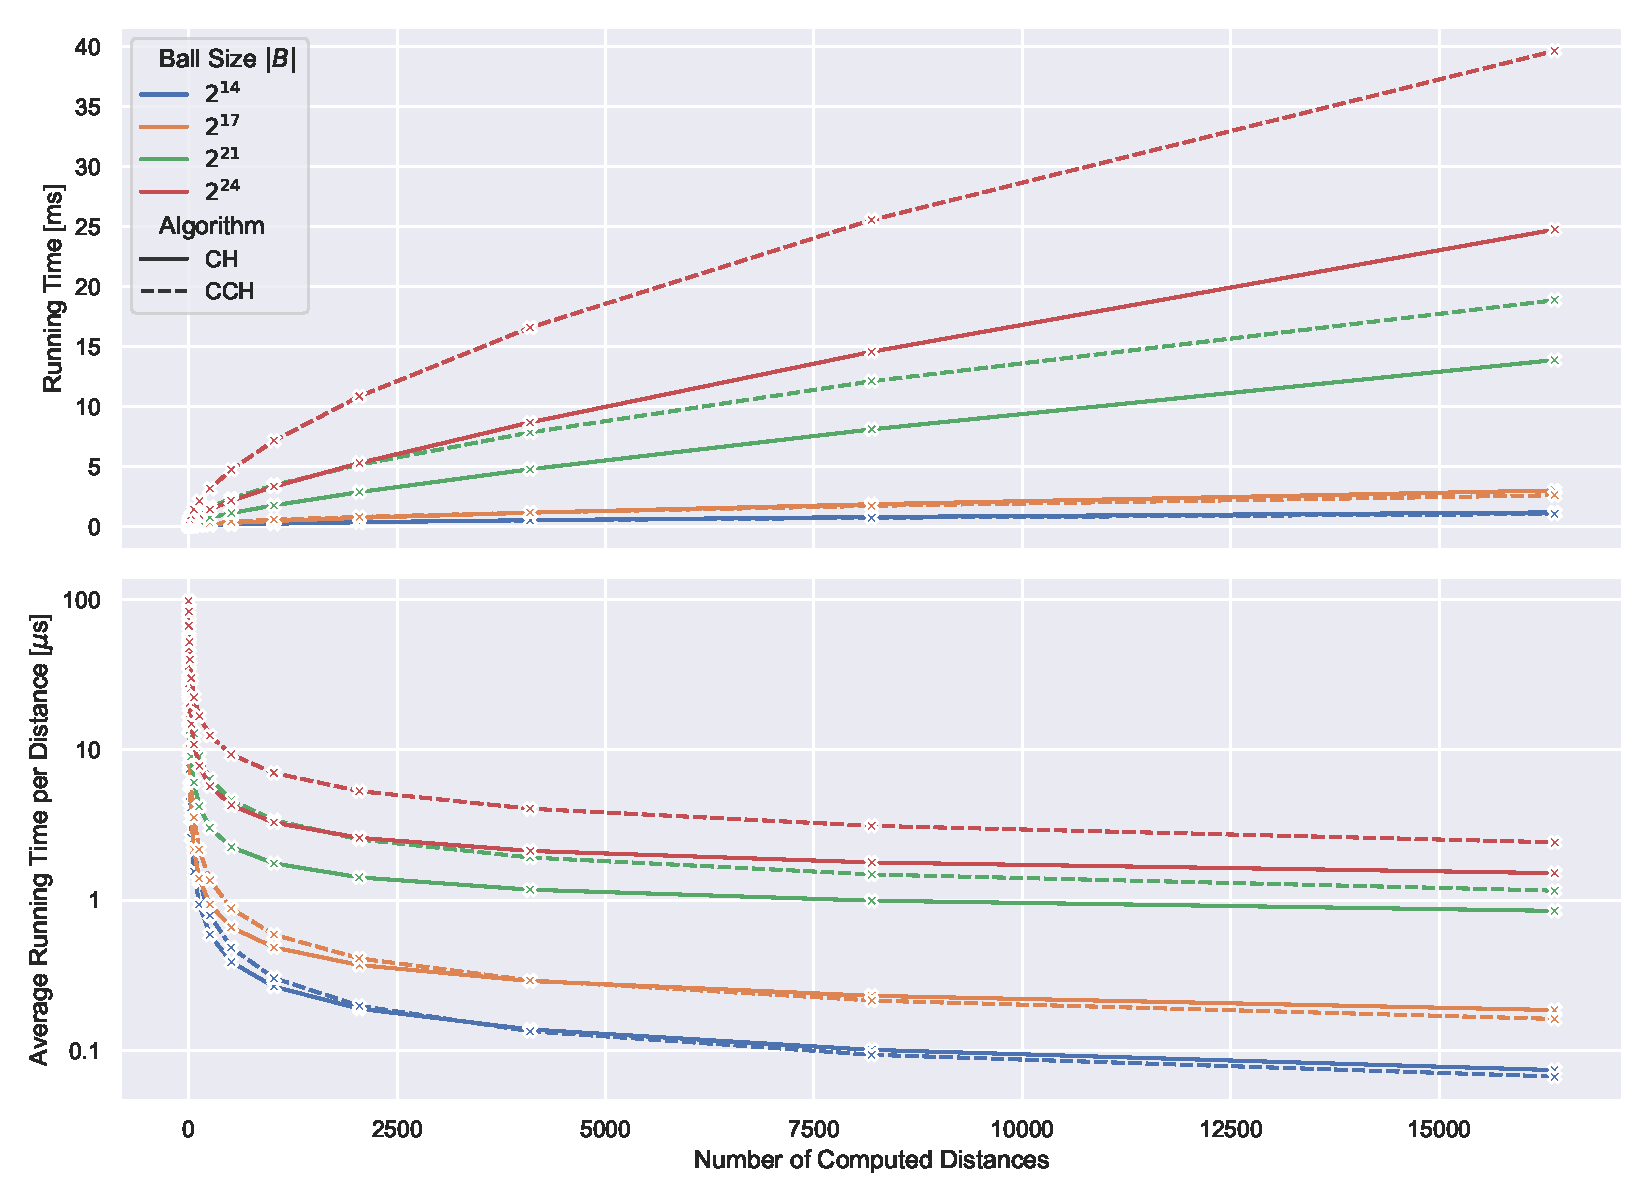
\includegraphics[width=\linewidth]{fig/lazy_rphast_inc.pdf}
\caption{
Average running times of incremental Lazy RPHAST while querying $|S| = 2^{14}$ from a ball of varying size $|B|$ on OSM Germany excluding selection times.
The upper figure contains the total elapsed running time.
The lower figure contains the averaged running time per source, i.e. $y/x$ from the upper figure.
Note the different y-axis scales and units.
}\label{fig:lazy_rphast_inc}
\Description{
Two line graphs with each eight lines for different ball sizes and algorithms.
The x-axis in both graphs is the number of vertices that were queried up to that point in the incremental query.
In each graph, all lines have a similar shape and appear as scaled variants of each other.
The bigger the ball size the slower the whole algorithm.
The CCH based variant is somewhat slower for the most part.
Only for small ball sizes it is marginally faster when computing distances for more than 4096 sources.
When the ball is the entire graph, the CH based variant takes around 2.5ms for the first 512 sources, 5ms for 2048 sources and 25ms for 16384 sources.
Conversely, the average time per query is around 100mus for the first few queries, then drops to around 5mus after 512 sources, down to 2mus after 16384 sources.
For the smallest ball size of 16384, everything is 1.5 orders of magnitude faster.
}
\end{figure}

To evaluate Lazy RPHAST in the incremental setting, we measure the elapsed running time after distances from $2^i$ sources were queried.
Figure~\ref{fig:lazy_rphast_inc} depicts the total elapsed time and the average running time to compute a single distance.
The first few distances are the most expensive ones since a lot of the CH search space has not been explored yet.
With around 100\,$\mu$s, the running times are comparable to standard CH queries.
For later queries, only little work remains to be done and the overhead per distance becomes almost constant depending on the ball size.

The performance difference between the CH and CCH based variant is interesting.
The CCH based variant can utilize the elimination tree for a more efficient implementation but the search space is denser.
This makes earlier queries more expensive and later queries cheaper.
With this trade-off, it depends on the ball size which variant is faster in terms of total running time.

\begin{figure}
\centering
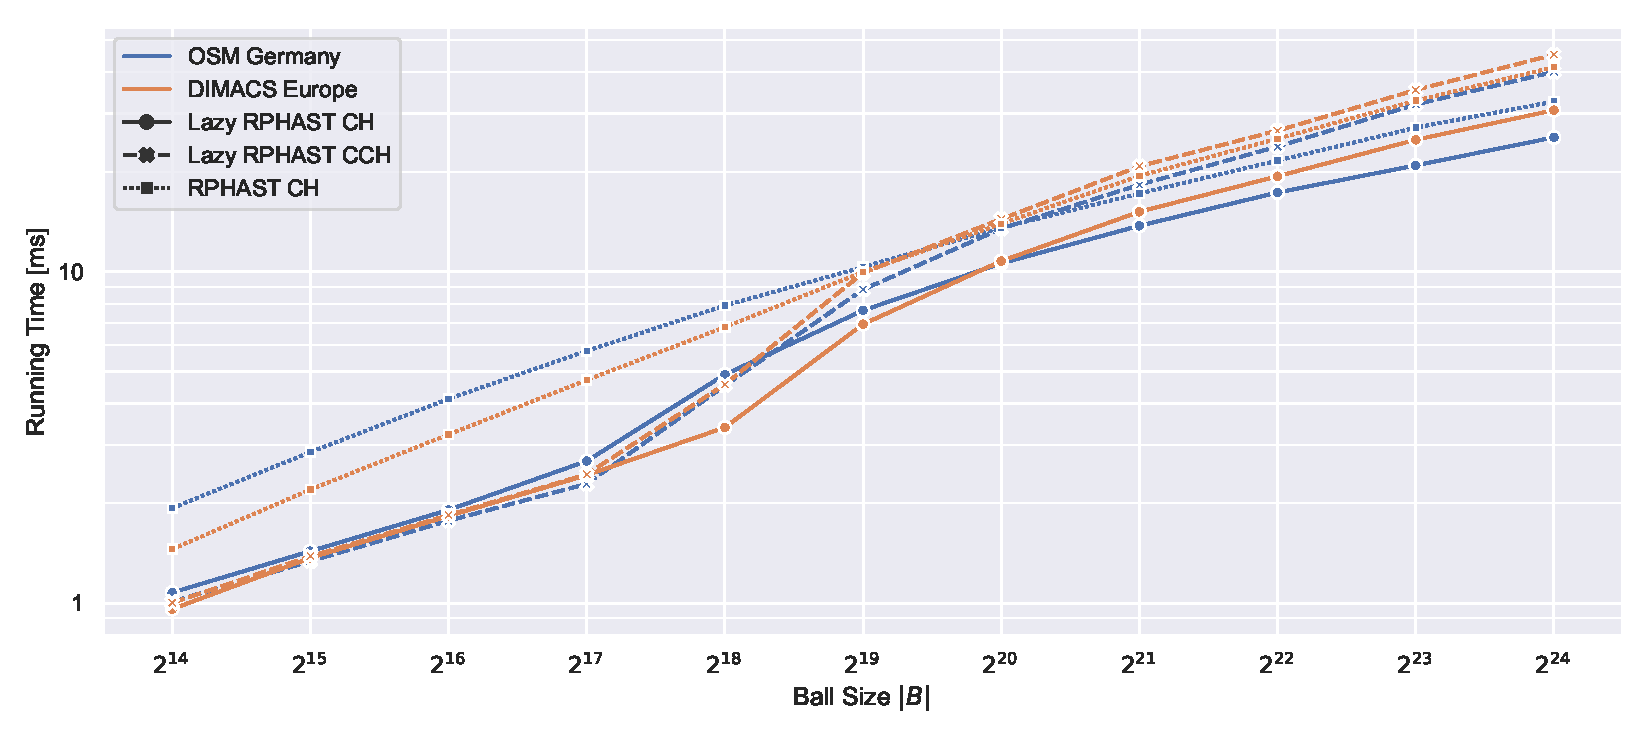
\includegraphics[width=\linewidth]{fig/lazy_rphast_many_to_one_both.pdf}
\caption{
Running times of (C)CH-based Lazy RPHAST for many-to-one queries with $|S| = 2^{14}$ sources picked from a ball of varying size $|B|$.
The running time includes the selection and the time to compute all distances.
}\label{fig:many_to_one}
\Description{
A double logarithmic line plot with four lines with similar shapes and absolute values.
Running times for both algorithms and graphs with a ball size of 16384 is around 1ms.
For a ball size of 2 to the 20 CH based variants need 10ms and CCH based variants slightly more.
For a ball size of 2 to the 24 CH based variants are at 30ms and CCH based variants slightly above 40ms.
}
\end{figure}

Despite the laziness being the distinguishing feature in Lazy RPHAST, the algorithm can still be used for non-incremental many-to-one queries.
Figure~\ref{fig:many_to_one} depicts average running times to compute distances between one target vertex and $2^{14}$ sources for different ball sizes.
The query generation methodology is the same as in the previous experiment.
As this is the same methodology also used in~\cite{delling_et_al:OASIcs:2011:3266}, we can relate our results to the performance of other one-to-many algorithms.
Keep in mind that algorithms like RPHAST optimize for a different setting than we do.
We can compare the performance for fixed $S$-$t$ terminal sets.
The difference is that with RPHAST one can efficiently compute distances from a different $t'$ to the same $S$ set while with Lazy RPHAST one can efficiently extend $S$ while $t$ stays the same.

When looking at total running times for a single many-to-one query including selection times, Lazy RPHAST delivers very competitive performance and is as fast if not faster than all algorithms evaluated in~\cite{delling_et_al:OASIcs:2011:3266}.
For example, Delling et al. report an average RPHAST running time of 1.97\,ms for selection and query combined for $|B| = 2^{14}$ and 28.52\,ms for $|B| = 2^{20}$ on DIMACS Europe.
Lazy RPHAST (on a CH) takes 0.96\,ms and 10.76\,ms respectively, to compute the same distances.
The CCH variant is slightly slower (1.00\,ms and 14.41\,ms) but still significantly faster than RPHAST.
While the numbers are not perfectly comparable due to different benchmark machines,\footnote{
According to the comparison methodology from~\cite{bdgmpsww-rptn-16} (see \url{https://i11www.iti.kit.edu/~pajor/survey/}), the machine used in~\cite{delling_et_al:OASIcs:2011:3266} (SPA-2) is about 30\% slower than ours (we obtained a score of 33\,159\,ms).
However, these scaling factors have to be interpreted very carefully.
They are obtained from one-to-all Dijkstra searches on continental-sized road networks.
This heavily emphasizes memory bandwidth while neglecting other critical factors such as CPU frequency and cache size and speed which are likely much more important for algorithms carefully tuned to exploit data locality.
} we can still conclude that Lazy RPHAST is a useful extension to RPHAST.
It allows efficiently handling dynamic source sets and is competitive in the setting where both the target and the source set change between queries.
% This is of course not a fair comparison since the approaches in~\cite{delling_et_al:OASIcs:2011:3266} are geared towards having one expensive selection phase and than many faster queries.
% When computing distances from different sources towards the same target set, RPHAST will outperform Lazy RPHAST.
% However, whenever the target set may change between queries, Lazy RPHAST offers a simple and fast alternative.

% \begin{figure}
% \centering
% 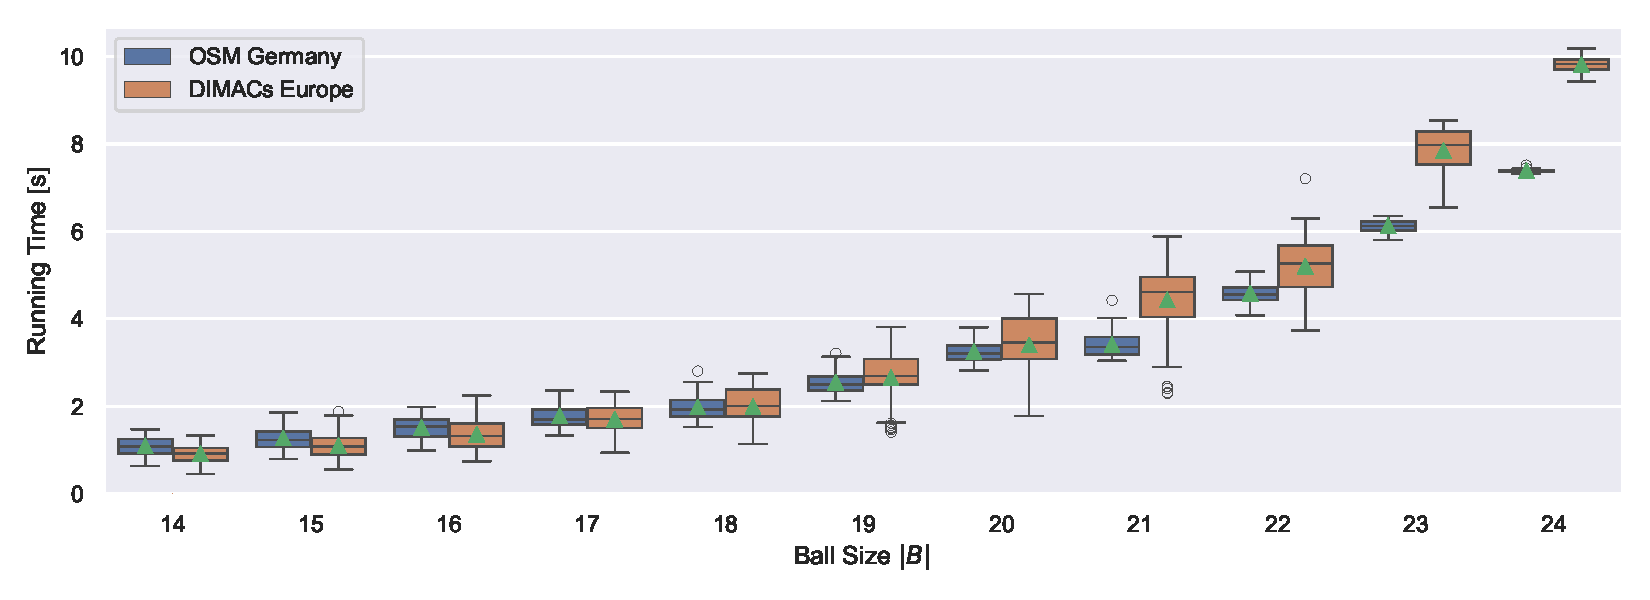
\includegraphics[width=\linewidth]{fig/lazy_rphast_many_to_many.pdf}
% \caption{
% Average running times of Lazy RPHAST for many-to-many queries with $|S| = |T| = 2^{14}$ sources and targets picked from a ball of varying size $|B|$ with standard deviation indicated as error bars.
% The lower part of the bars indicates the running time of the Bucket CH subphase.
% }\label{fig:many_to_many}
% \end{figure}

% Applying Lazy RPHAST to the many-to-many problem results in running times as depicted in Figure~\ref{fig:many_to_many}.
% The results are again at least competitive to the performance reported for SSE RPHAST in~\cite{delling_et_al:OASIcs:2011:3266}.
% % TODO konkrete zahlen?
% The Bucket CH based first query phase of our implementation takes between half of the total query time for $|B| = 2^{14}$ and a tenth of the time for $|B| = 2^{24}$.
% It is worth noting that contrary to SSE RPHAST, we did not explicitly utilize SIMD instructions.
% However, the code for Lazy RPHAST on an arrays of distances can be trivially vectorized by the compiler.
% We confirmed that the code was indeed vectorized by inspecting the generated assembly.

% \subsubsection{k-Nearest-Neighbor Queries with CCH}

% One-to-many queries appear in many extended applications as a subproblem.
% In some of these cases Lazy RPHAST can be used to achieve significant speed-ups with surprisingly little effort.
% One such example are k-Nearest-Neighbor Queries with CCH~\cite{buchhold_et_al:LIPIcs.SEA.2021.18}.
% There, shortest distances are computed repeatedly from the same source to boundary vertices of a cell of vertices.
% On our suggestion, the authors integrated Lazy RPHAST into their algorithm which took only a couple of lines of code\footnote{\url{https://github.com/vbuchhold/routing-framework/commit/c739dc8e81}}.
% We reran their improved experiments and include the results in our appendix.
% Briefly summarized, integrating Lazy RPHAST into this algorithm decreased running times by up to 15 times depending on the distribution of the target set for almost no effort.
% This demonstrates that Lazy RPHAST is not only useful as an A* potential but also applicable in other contexts.

\subsection{(C)CH-Potentials Heuristic}

\begin{figure}
\centering
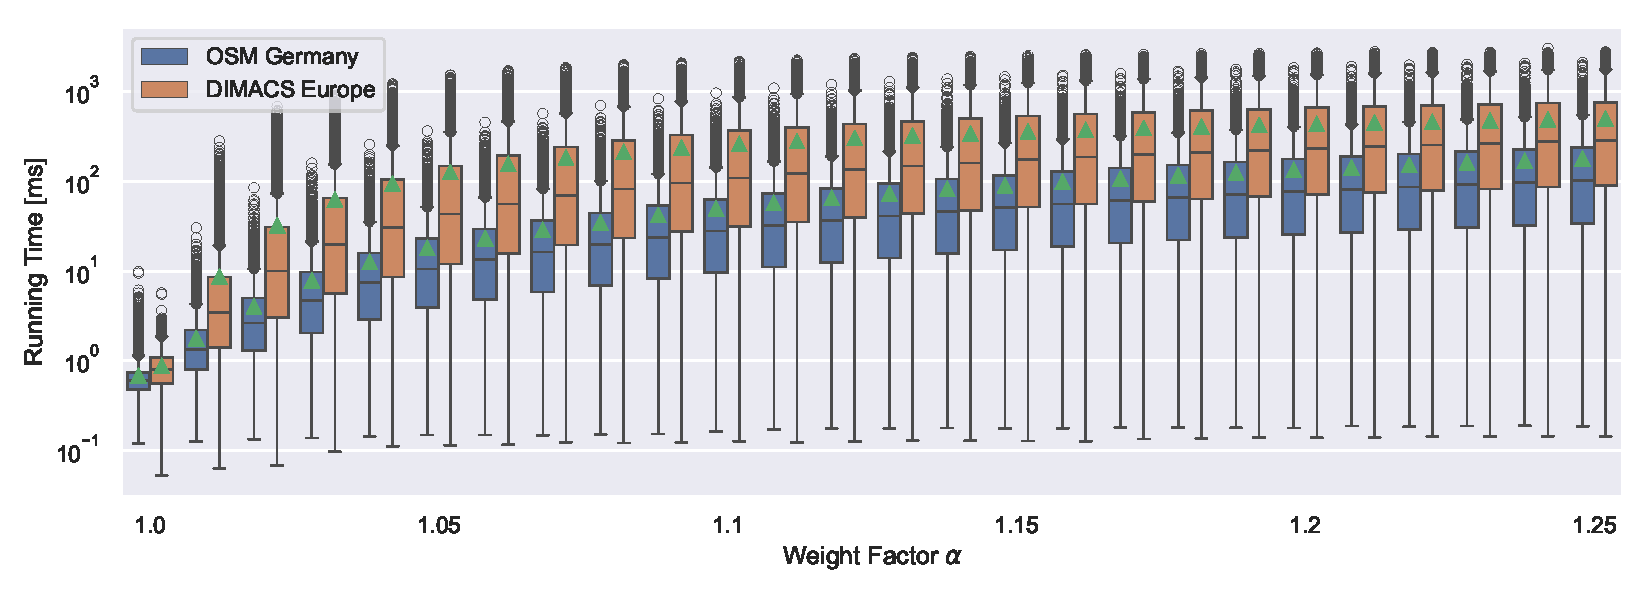
\includegraphics[width=\linewidth]{fig/scaled_weights.pdf}
\caption{
Running times on a logarithmic scale for queries on OSM Ger with scaled edge weights $w_q = \alpha \cdot w_\ell$.
The boxes cover the range between the first and third quartile.
The band in the box indicates the median, the diamond the mean.
The whiskers cover 1.5 times the interquartile range.
All other running times are indicated as outliers.
}\label{fig:scaled_weights}
\Description{Fully described in the text.}
\end{figure}

The performance of A* depends on the tightness of the heuristic and the overhead of evaluating the heuristic.
CH-Potentials computes optimal distance estimates with respect to $w_\ell$.
However, for most applications, there will be a gap between $w_q$ and $w_\ell$ (otherwise one could use CH without A*).
We evaluate the impact of the difference between $w_q$ and $w_\ell$ on the performance of A*.
The lower bound $w_\ell$ is set to the free-flow travel time.
The query weights $w_q$ are set to $\alpha \cdot w_\ell$, where $\alpha\ge 1$.
% When $\alpha = 1$, the heuristic is tight.
Increasing $\alpha$ degrades the heuristic's quality.
Figure~\ref{fig:scaled_weights} depicts the results.
Clearly, $\alpha$ has significant influence on the running time.
Average running times range from below a millisecond to a few hundred milliseconds depending on $\alpha$.
Up to around $\alpha = 1.1$ the running time grows quickly.
For $\alpha > 1.1$, the growth slows down.
This illustrates both the strengths and limits of our approach and goal-directed search in general.
CH-Potentials can only achieve competitive running times if the application allows for sufficiently tight lower bounds at preprocessing time.

We observe that the running times for a fixed $\alpha$ vary strongly.
This is an interesting observation, as with uniform source and target sampling, nearly all queries are long-distance.
The query distance is thus not the reason.
After some investigation, we concluded that this is due to non-uniform road network density.
Some regions have more roads per area than others.
The number of vertices explored by A* depends on the density of the search space area.
As the density varies, the running times vary.

\begin{table}
\centering
\caption{
Average query running times and number of queue pushes with different heuristics and optimizations on OSM Ger with $w_q = 1.05 \cdot w_\ell$.
The BCC, Deg2 and Deg3 columns indicate which optimizations from Section~\ref{sec:low-deg-improvment} were used.
}\label{tab:building_blocks}
\begin{tabular}{clllrrrrr}
\toprule
       & BCC & Deg2 & Deg3 & Zero & ALT & CH & CCH & Oracle \\
\midrule
\multirow{4}{*}{\rotatebox[origin=c]{90}{\shortstack{Running\\time [ms]}}} & \xmark &        \xmark &        \xmark &  2\,133.0 &  317.9 &   47.9 &   54.4 &    34.3 \\
                                                                                    & \cmark &        \xmark &        \xmark &  1\,355.3 &  233.9 &   36.3 &   38.5 &    24.8 \\
                                                                                    & \cmark &         \cmark &        \xmark &   753.4 &  122.6 &   19.5 &   22.1 &    12.7 \\
                                                                                    & \cmark &         \cmark &         \cmark &   580.7 &   90.8 &   15.9 &   18.1 &    10.1 \\
\addlinespace
\multirow{4}{*}{\rotatebox[origin=c]{90}{\shortstack{Queue\\pushs[$\cdot 10^3$]}}} & \xmark &        \xmark &        \xmark &  8\,087.1 &  863.1 &  137.1 &  137.1 &   137.1 \\
                                                                                    & \cmark &        \xmark &        \xmark &  6\,298.2 &  685.7 &  112.7 &  112.7 &   112.7 \\
                                                                                    & \cmark &         \cmark &        \xmark &  2\,901.4 &  303.4 &   43.3 &   43.3 &    43.3 \\
                                                                                    & \cmark &         \cmark &         \cmark &  1\,681.4 &  179.7 &   26.8 &   26.8 &    26.8 \\
\bottomrule
\end{tabular}


\end{table}

Table~\ref{tab:building_blocks} depicts the performance of unidirectional A* with different heuristics and optimizations on OSM Ger with $w_q = 1.05 \cdot w_\ell$.
The factor 1.05 was chosen to resemble realistic problem settings where goal-directed search can achieve reasonable speedups (compare to Table~\ref{tab:applications}).
We compare (C)CH-Potentials to three other heuristics.
The first heuristic is the \emph{Zero} heuristic where $h(v)$ is $0$ for all vertices $v$.
This corresponds to using Dijkstra's algorithm.
Secondly, we compare against our own implementation of ALT~\cite{gw-cppsp-05}.
We use 16 landmarks generated with the avoid strategy~\cite{gw-cppsp-05} and activate all during every query.
Finally, we compare against a hypothetical \emph{Oracle-A*} heuristic.
This heuristic has instant access to a shortest distance array with respect to $w_\ell$, i.e. it is faster than the fastest heuristic possible in our model.
We fill this array before each query using a reverse Dijkstra search from the target vertex but do not include the running time for this step.
Thus, the reported running times of Oracle-A* do \emph{not} account for any heuristic evaluation.
(C)CH-Potentials computes the same distance estimates, but the heuristic evaluation has some overhead.
Comparing against Oracle-A* allows us to measure this overhead.
No other heuristic, which only has access to the preprocessing weights, can be faster than Oracle-A*.

We observe that the number of queue pushes roughly correlates with running time.
As (C)CH-Potentials and Oracle-A* have the same heuristic values, the number of queue pushes are by construction equal.
Each optimization reduces both queue pushes and running times.
All optimizations yield a combined speedup of around 3.
% Skipping degree three vertices has the smallest impact.
(C)CH-Potentials outperforms ALT by a factor of between six and seven and settle correspondingly fewer vertices.
This is not surprising, since ALT computes worse distance estimates.
In contrast, CH-Potentials already computes exact distances with respect to $w_\ell$.
The number of popped vertices is the same for CH-Potentials, CCH-Potentials and Oracle-A*.
The only difference between (C)CH-Potentials and Oracle-A* is the overhead of the heuristic evaluation.
This overhead leads to a slowdown of around 1.6.
Thus, CH-Potentials is already very close to the best possible heuristic in this model.
% Very interesting is the comparison with Oracle-A*.
% Our algorithm is only 1.6 times slower than accessing the exact $w_\ell$ distances instantly from a precomputed array.
This means that no competing algorithm such as ALT or CPD-Heuristics can be significantly faster.
CCH-Potentials is slightly slower than CH-Potentials because they use a weight independent vertex importance order.
This enables CCH-Potentials to support a customization whereas CH-Potentials cannot.

\subsection{Bidirectional A*}

\begin{table}
\centering
\caption{
Performance of different variants of bidirectional A* on OSM Ger with $w_q = 1.05 \cdot w_\ell$.
All variants alternate between the forward and the backward search.}
\label{tab:bidir_pruning}
\begin{tabular}{c@{\hskip6pt}c@{\hskip3pt}crrrrrrrr}
\toprule
 &  &  & \multicolumn{5}{c}{Running time [ms]} & \multicolumn{3}{c}{Queue pushes [$\cdot 10^3$]} \\ \cmidrule(lr){4-8} \cmidrule(lr){9-11}
Low Deg.      & Bidirectional & New & \multirow{2}{*}{Zero} & \multirow{2}{*}{ALT} & \multirow{2}{*}{CH} & \multirow{2}{*}{CCH} & \multirow{2}{*}{Oracle} & \multirow{2}{*}{Zero} & \multirow{2}{*}{ALT} & (C)CH/ \\
Opt. & Potential     & Pruning  & & & & & & & & Oracle \\
\midrule
              \xmark &   Average &            \xmark &           1\,441.41 & 126.46 &  62.61 &  53.91 &  37.29 &                    4\,493.97 &  292.01 &       125.16 \\
              \xmark &   Average &             \cmark &           1\,451.96 & 128.20 &  62.48 &  54.28 &  38.89 &                    4\,491.56 &  290.92 &       125.08 \\
              \xmark & Symmetric &            \xmark &           5\,779.64 & 795.56 & 122.70 & 111.78 &  88.66 &                   16\,042.82 & 1\,688.60 &       259.78 \\
              \xmark & Symmetric &             \cmark &           1\,453.58 & 261.80 &  59.22 &  51.97 &  37.37 &                    4\,491.56 &  624.25 &       116.71 \\
\addlinespace
\cmark &   Average &            \xmark &            365.82 &  33.22 &  19.34 &  18.66 &   9.96 &                     916.15 &   57.27 &        23.60 \\
\cmark &   Average &             \cmark &            369.51 &  33.37 &  19.54 &  18.88 &   9.98 &                     908.55 &   56.09 &        23.25 \\
\cmark & Symmetric &            \xmark &           1\,512.48 & 241.27 &  40.98 &  38.99 &  26.36 &                    3\,317.81 &  334.90 &        44.67 \\
\cmark & Symmetric &             \cmark &            368.94 &  72.67 &  21.54 &  20.39 &  11.22 &                     908.55 &  123.77 &        20.72 \\
\bottomrule
\end{tabular}


\end{table}

In this section, we investigate the performance of bidirectional A*.
We first evaluate different variants of bidirectional A* in Table~\ref{tab:bidir_pruning} and~\ref{tab:bidir_switching} then compare the best ones against unidirectional A* in Table~\ref{tab:bidir}.
Table~\ref{tab:bidir_pruning} studies the impact of our improved pruning and the low degree optimizations.
As observed in the previous section, enabling the low degree optimization achieves a speedup by roughly a factor of three.
Symmetric bidirectional A* without our improved pruning has the worst performance.
Enabling the improved pruning significantly improves the performance of symmetric bidirectional A*.
For all heuristics except ALT, symmetric A* with the improved pruning has smaller search spaces than the average potential and very similar running times.
Without the low degree improvements, the improved symmetric variant is marginally faster and with the low degree improvements the average potential remains slightly faster.
This is due to the reduced impact of the heuristic evaluation overhead with the low degree optimizations.
Enabling the improved pruning for the average potential marginally reduces the search space size and slightly increases running times.

\begin{table}
\centering
\caption{
Performance of different direction selection criteria of bidirectional A* on OSM Ger with different query weights.
The symmetric variant uses the improved pruning, the average variant does not.
All variants use all low degree optimizations.
}\label{tab:bidir_switching}
\begin{tabular}{cccrrrrrrrr}
\toprule
 &  &  & \multicolumn{5}{c}{Running time [ms]} & \multicolumn{3}{c}{Queue pushs [$\cdot 10^3$]} \\ \cmidrule(lr){4-8} \cmidrule(lr){9-11}\multirow{2}{*}{$w_q$} & Bidirectional & Choose    & \multirow{2}{*}{Zero} & \multirow{2}{*}{ALT} & \multirow{2}{*}{CH} & \multirow{2}{*}{CCH} & \multirow{2}{*}{Oracle} & \multirow{2}{*}{Zero} & \multirow{2}{*}{ALT} & (C)CH/ \\
 & Potential     & Direction & & & & & & & & Oracle \\
\midrule
\multirow{4}{*}{$w_{\ell}$} &   Average &               Alternating &            373.18 & 12.83 &  0.79 &  1.13 &   0.18 &                     916.15 &  23.08 &         0.60 \\
           &   Average &                  Min. Key &            406.35 & 13.68 &  1.44 &  1.75 &   0.56 &                     986.40 &  26.39 &         1.15 \\
           & Symmetric &               Alternating &            376.72 & 40.19 &  0.69 &  0.92 &   0.19 &                     908.55 &  76.61 &         0.57 \\
           & Symmetric &                  Min. Key &            427.51 & 50.46 &  1.77 &  1.99 &   0.83 &                     978.62 &  99.62 &         1.44 \\
\addlinespace
     \multirow{4}{*}{$w_{\ell} \cdot 1.05$} &   Average &               Alternating &            365.82 & 33.22 & 19.34 & 18.66 &   9.96 &                     916.15 &  57.27 &        23.60 \\
           &   Average &                  Min. Key &            391.70 & 38.06 & 21.76 & 20.44 &  11.30 &                     986.41 &  67.65 &        26.42 \\
           & Symmetric &               Alternating &            368.94 & 72.67 & 21.54 & 20.39 &  11.22 &                     908.55 & 123.77 &        20.72 \\
           & Symmetric &                  Min. Key &            394.38 & 84.84 & 27.28 & 24.64 &  14.53 &                     978.63 & 145.28 &        24.82 \\
\addlinespace
   \multirow{4}{*}{\shortstack{$w_{\ell} \cdot 1.5$ if\\ $v <$ 80kph}} &   Average &               Alternating &            361.83 & 19.50 & 10.92 & 10.94 &   5.34 &                     845.06 &  34.03 &        13.25 \\
           &   Average &                  Min. Key &            391.47 & 31.65 & 21.05 & 20.10 &  11.00 &                     917.13 &  52.23 &        23.78 \\
           & Symmetric &               Alternating &            364.55 & 37.33 & 11.89 & 11.75 &   6.00 &                     836.44 &  57.93 &        11.53 \\
           & Symmetric &                  Min. Key &            395.04 & 54.90 & 23.36 & 22.48 &  12.54 &                     908.12 &  84.33 &        22.01 \\
\bottomrule
\end{tabular}


\end{table}

Table~\ref{tab:bidir_switching} shows the performance of bidirectional A* with different strategies to decide whether to advance the forward or the backward search next.
The results clearly show that alternating the directions is always superior.
Selecting the direction by minimum queue key may lead to huge imbalances in the progress of the searches.
This causes the searches to meet later and the total search space to grow significantly.

\begin{table}
\centering
\caption{
Performance of bidirectional and unidirectional A* on OSM Ger with different query weights.
The symmetric variant uses the improved pruning, the average variant does not.
All variants use all low degree optimizations.
}\label{tab:bidir}
\begin{tabular}{ccrrrrrrrr}
\toprule
 &  & \multicolumn{5}{c}{Running time [ms]} & \multicolumn{3}{c}{Queue pushes [$\cdot 10^3$]} \\ \cmidrule(lr){3-7} \cmidrule(lr){8-10}\multirow{2}{*}{$w_q$} & & \multirow{2}{*}{Zero} & \multirow{2}{*}{ALT} & \multirow{2}{*}{CH} & \multirow{2}{*}{CCH} & \multirow{2}{*}{Oracle} & \multirow{2}{*}{Zero} & \multirow{2}{*}{ALT} & (C)CH/ \\
 & & & & & & & & & Oracle \\
\midrule
\multirow{3}{*}{$w_{\ell}$} & Unidirectional &            584.87 & 43.02 &  0.47 &  0.64 &   0.16 &                    1\,674.35 &  96.21 &         0.66 \\
        & Average &            373.18 & 12.83 &  0.79 &  1.13 &   0.18 &                     916.15 &  23.08 &         0.60 \\
        & Symmetric &            376.72 & 40.19 &  0.69 &  0.92 &   0.19 &                     908.55 &  76.61 &         0.57 \\
\addlinespace
\multirow{3}{*}{$w_{\ell} \cdot 1.05$} & Unidirectional &            580.66 & 90.79 & 15.91 & 18.09 &  10.06 &                    1\,681.39 & 179.66 &        26.78 \\
        & Average &            365.82 & 33.22 & 19.34 & 18.66 &   9.96 &                     916.15 &  57.27 &        23.60 \\
        & Symmetric &            368.94 & 72.67 & 21.54 & 20.39 &  11.22 &                     908.55 & 123.77 &        20.72 \\
\addlinespace
\multirow{3}{*}{\shortstack{$w_{\ell} \cdot 1.5$ if\\ speed \\< 80kph}} & Unidirectional &            637.24 & 96.62 & 21.78 & 21.37 &  14.62 &                    1\,674.26 & 171.02 &        36.54 \\
        & Average &            361.83 & 19.50 & 10.92 & 10.94 &   5.34 &                     845.06 &  34.03 &        13.25 \\
        & Symmetric &            364.55 & 37.33 & 11.89 & 11.75 &   6.00 &                     836.44 &  57.93 &        11.53 \\
\bottomrule
\end{tabular}


\end{table}

In Table~\ref{tab:bidir} we investigate the effectiveness of bidirectional search compared to unidirectional search depending on the query weights.
Interestingly, only the zero heuristic and ALT consistently achieve speedups through bidirectional search on all query weights.
With $w_q = w_{\ell}$, unidirectional CH-Potentials is already optimal and only traverses the shortest path.
Here, bidirectional search will only introduce unnecessary overhead.
When query weights are scaled up uniformly, bidirectional search achieves some search space reduction, but it is not enough to significantly reduce running times due to the overhead of running a second search.
This changes drastically when the query weight increases are applied non-uniformly in the third scenario.
Here only weights with a speed less than 80\,kph were scaled up.
This touches only the beginning and end of most shortest paths between randomly chosen vertices.
The middle part of the shortest paths will typically use faster edges like highways.
In this case, bidirectional (C)CH-Potentials is a factor of two faster than the unidirectional variant.
The reason for this is that the search space of a unidirectional search expands greatly while exploring the end of the path to the target where the reduced weights are bad.
In contrast, the bidirectional searches meet in the middle of the shortest path where the reduced weights are close to zero and thus avoid this expansion.
This is also the reason why ALT behaves like this for all query weights.
By construction, the ALT heuristic has better reduced weights for edges which are on many shortest paths like highways.
Conversely, unimportant edges have bad reduced weights.
This makes bidirectional search so critical for ALTs performance.
In contrast, having a potential as tight as CH-Potentials makes bidirectional search in many scenarios unnecessary.
Bidirectional search for CH-Potentials only pays off when the reduced weights are bad around the terminals.

\subsection{Applications}

\begin{table*}
\centering
\caption{
CH-Potentials performance for different route planning applications.
Depending on the problem we apply unidirectional or bidirectional CH-Potentials (CH U or CH B) or CCH-Potentials (CCH U/B).
We report average running times and number of queue pushes.
We also report the average length increase, that is how much longer the final shortest distance is compared to the lower bound.
Finally, we report the average running time of Dijkstra's algorithm as a baseline and the speedup over this baseline.
}\label{tab:applications}
\begin{tabular}{llrrrrrr}
\toprule
 & & &   Running &                Queue &     Length & Dijkstra & Speedup \\ & & & time [ms] & $[\cdot 10^3]$ & incr. [\%] &     [ms] &         \\
\midrule
DIMACS Eur & Unmodified $w_q = w_{\ell}$ & CH U &              0.9 &              1.1 &       0.0 &                    2106.0 &   2405.8 \\
\addlinespace
OSM Ger & Unmodified $w_q = w_{\ell}$ & CH U &              0.6 &              0.5 &       0.0 &                    2182.6 &   3795.4 \\[2pt]
        & No Tunnels & CH U &             29.2 &             46.8 &       5.2 &                    2198.0 &     75.2 \\
        &    & CH B &             33.4 &             35.7 &       5.2 &                    2198.0 &     65.8 \\[2pt]
        & No Highways & CH U &            378.7 &            583.8 &      42.5 &                    1992.5 &      5.3 \\
        &    & CH B &            433.1 &            481.6 &      42.5 &                    1992.5 &      4.6 \\[2pt]
        & Live & CH U &            129.4 &            193.9 &      15.0 &                    2119.3 &     16.4 \\
        &    & CH B &            193.6 &            188.8 &      15.0 &                    2119.3 &     10.9 \\
        &    & CCH U &              1.1 &              0.8 &       0.0 &                    2119.3 &   1920.4 \\[2pt]
        & Turns & CH U &              3.0 &              5.7 &       1.1 &                    4708.2 &   1556.0 \\
        &    & CH B &              1.1 &              0.8 &       1.1 &                    4708.2 &   4223.8 \\[2pt]
        & Live + Turns & CCH U &              4.8 &              8.8 &       1.0 &                    4621.8 &    959.7 \\
        &    & CCH B &              2.1 &              1.6 &       1.1 &                    4621.8 &   2168.1 \\[2pt]
        & TD & CH U &            120.8 &            104.4 &      12.3 &                    3133.7 &     25.9 \\
        & TD + Live & CH U &            198.3 &            170.3 &      20.7 &                    3436.5 &     17.3 \\
        & TD + Live + Turns & CH U &            474.2 &            657.8 &      21.7 &                    6420.5 &     13.5 \\
\addlinespace
TDEur17 & TD & CH U &             80.4 &             79.8 &       3.9 &                    3454.3 &     43.0 \\
TDEur20 & TD & CH U &             97.7 &             72.8 &       4.2 &                    5060.2 &     51.8 \\
TDGer06 & TD & CH U &              4.2 &              6.4 &       3.1 &                     603.5 &    144.2 \\
\bottomrule
\end{tabular}


\end{table*}

Table~\ref{tab:applications} depicts the running times of (C)CH-Potentials in various applications, such as those described in Section~\ref{sec:applications}.
We report speedups compared to extensions of Dijkstra's algorithm for each application respectively.
We start with the base case where $w_q = w_\ell$.
This is the problem variant solved by the basic CH algorithm.
CH achieves average query running times of 0.16\,ms on OSM Ger.
CH-Potentials is roughly four times slower but still achieve a huge speedup of 3795 over Dijkstra.
Such large speedups are typical for CH.
This shows that CH-Potentials gracefully converges toward CH in the $w_q = w_\ell$ special case.
On DIMACS Europe, the average degree is somewhat higher which makes the low-degree optimizations less effective which leads to more queue operations and a slightly slower running time.

In the other scenarios, the performance of CH-Potentials strongly depends on the quality of the heuristic.
We measure this quality using the length increase of $w_q$ compared to $w_\ell$.
Forbidding highways results in the largest length increase and in the smallest speedup.
The other extreme are turn restrictions.
They have only a small impact on the length increase.
The achieved speedups are therefore comparable to CH speedups.
Since turn costs and restrictions appear mostly in the beginning and end of shortest-paths and not in the middle on highways, utilizing bidirectional search results in even better speedups.
Mapbox live traffic has a length increase of around 15\%, which yields running times of 130\,ms.
Applying bidirectional CH-Potentials in this case is, in fact, detrimental to the performance because the bad reduced edge weights appear in the middle of shortest paths.
The same is the case for forbidden tunnels or highways.
Applying CCH-Potentials customized to the current traffic (or the metric with forbidden edges) to these problems yields running times similar to the unmodified case and speedups of more than three orders of magnitude.
With bidirectional CCH-Potentials, one can easily additionally support turn costs and still have running times of a few milliseconds without any adjustments to the customization.

The length increase of Mapbox traffic predictions is about 12.3\%, and results in a running time of 120\,ms.
The speedup in the predicted scenario is larger than in the live setting, as the travel time function evaluations slow down Dijkstra's algorithm.
Combining predicted and live traffic results in a running time of around 200\,ms.
Further adding turn restrictions, significantly increases the running times.
This increase is mostly due to the BCC optimization of Section~\ref{sec:largested-biconnected-component} becoming ineffective when considering turns.
It is not due to the length increase of using turns.
With everything activated, our algorithm still has a speedup of 13.5 over the baseline.
Interestingly, the PTV traffic predictions have a much smaller length increase than the Mapbox predictions.
This results in somewhat smaller running times of our algorithm.

\paragraph{Comparison with Related Work}

While the query running times reported in Table~\ref{tab:applications} are decent in many settings, they are not competitive to techniques tailored to specific applications.
In the simple $w_q = w_{\ell}$ setting, Hub Labels can be used to answer queries in less than a microsecond~\cite{DBLP:conf/wea/DellingGW13}, more than three orders of magnitude faster than with CH-Potentials.
Live traffic and arbitrary weight functions can be handled with CCH resulting in query times of around a 0.1\,ms~\cite{DBLP:journals/jea/Buchhold0W19}.
CCH can also be adjusted to turn costs.
With some algorithmic adjustments to the preprocessing~\cite{bwzz-cchtc-20}, query times around an order of magnitude faster than CCH-Potentials are possible (0.3\,ms compared to 2.1\,ms with CCH-Potentials).
For time-dependent routing, CATCHUp~\cite{swz-sfert-21} achieves query times more than an order of magnitude faster than CH-Potentials (6.3\,ms compared to our 97.7\,ms).
Again, these numbers are not perfectly comparable due to different benchmark machines.
Nevertheless, the overall picture is clear enough.
However, the advantage of the CH-Potentials framework over these fine-tuned techniques is that it is unified and flexible approach which can handle all these applications without any adjustments to the preprocessing.
Further, CH-Potentials preprocessing times are at least an order of magnitude faster than approaches like CATCHUp (sequentially more than four hours on TDEur20 compared to five minutes with CH-Potentials) and require significantly less memory (Hub Labels, for example, needs 20\,GiB on DIMACS Europe, compared to around 750\,MiB with CH-Potentials, see Table~\ref{tab:graphs}).
Finally, to the best of our knowledge, for problem settings such as the combination of predicted and live traffic, there simply does not exist any exact technique able to handle this setting, let alone additionally integrating turn costs.
The key achievement of CH-Potentials is that problem extensions can be integrated by trading query performance rather than developing new algorithms.

% \subsubsection{Alternative Routes}

% Our implementation of the penalty method reproduces the qualitative results reported in~\cite{kobitzsch2015alternative} (for random queries on DIMACS Europe we on average achieve a total distance of 2.93, an average distance of 1.04, 5.57 decision edges and a success rate of 98.7\% with 6.7 iterations).
% The average running times to compute an alternative graph are 1.37\,s on DIMACS Europe and 0.85\,s on OSM Germany.
% These running times are roughly one order of magnitude slower than the results achieved by Kobitzsch.
% The simpler penalty routes approach is much faster and takes only 156\,ms on DIMACS Europe and 66\,ms on OSM Germany.
% This is two orders of magnitude faster than the running times reported in~\cite{adgw-arrn-13} which is not surprising since their implementation uses an unaccelerated Dijkstra.
% Due to the advanced penalization schema, our average qualitative results differ from~\cite{adgw-arrn-13}: the success rate is with 96.8\% slightly higher, the UBS with around 9\% slightly worse, the sharing is with 42\% somewhat higher but the local optimality, which was the weakest point in the original approach, with 21\% significantly better.
% Finding these alternatives takes only 1.44 iterations on average.
% This makes CH-Potential-based penalty routes a simple and feasible practical approach to compute alternative routes.

\section{Conclusion}
\label{sec:conclusion}

In this article, we introduced CH-Potentials, a fast, exact, and flexible two-phase routing framework based on A* and CH.
The approach can handle a multitude of complex, integrated routing scenarios with very little implementation complexity and without any changes to the preprocessing algorithms.
CH-Potentials provides \emph{exact} distances with respect to lower bound weights known at preprocessing time as an A* heuristic.
Thus, the query performance of CH-Potentials crucially depends on the availability of good lower bounds in the preprocessing phase.
Our experiments show, that this availability highly depends on the application.
We also show that the overhead of our heuristic is within a factor 1.6 of a hypothetical A*-heuristic that can instantly access lower bound distances.
Achieving significantly faster running times could still be possible in variations of the problem setting.
The core building block of our approach is Lazy RPHAST, a new CH query variant for the incremental many-to-one problem.
We showed that it also delivers competitive performance for many-to-one problems.
This leads to multiple avenues for future research.

Dropping the provable exactness requirement using a setup similar to anytime A*~\cite{DBLP:conf/aaai/ZhouH02,DBLP:conf/nips/LikhachevGT03} would be interesting.
Another promising research avenue would be to investigate graphs other than road networks.
A lot of research into grid maps exists including a series of competitions called GPPC~\cite{DBLP:conf/socs/SturtevantTTUKS15}.
Hierarchical techniques have been shown to work well on these graphs~\cite{DBLP:conf/aaai/UrasK14}.
It might also be worthwhile to apply CH-Potentials to even more routing applications, for example to the shortest $\epsilon$-smooth path problem~\cite{dss-tarrn-18} or the problem of computing alternative routes~\cite{adgw-arrn-13,bdgs-argrn-11,kobitzsch2015alternative}.
Many-to-one problems also appear as subproblems in other routing algorithms, for example in nearest neighbor computations~\cite{buchhold_et_al:LIPIcs.SEA.2021.18}.
Investigating whether Lazy RPHAST can be used to improve these algorithms appears to be a worthwhile direction for future research.
Studying the performance of Lazy RPHAST in a many-to-many context would also be interesting.

\section*{Acknowledgements}
This article is the extended version of our conference paper ``A Fast and Tight Heuristic for A* in Road Networks''~\cite{strasser_et_al:LIPIcs.SEA.2021.6}.

%%
%% Bibliography
%%

%% Please use bibtex,

\bibliographystyle{ACM-Reference-Format}
\bibliography{references}

% \appendix

% \section{Improved Results for k-Nearest-Neighbor Queries on CCH}

% In this section, we report the results of the k-Nearest-Neighbor Queries on CCH with Lazy RPHAST.
% The authors of~\cite{buchhold_et_al:LIPIcs.SEA.2021.18} provide the code for their algorithm and their experiments on Github\footnote{\url{https://github.com/vbuchhold/routing-framework}}.
% This includes the code for both the old version and the new one improved with Lazy RPHAST.
% We reran the experiments performed for~\cite{buchhold_et_al:LIPIcs.SEA.2021.18} in both the old and the new configuration on our machine.
% In the results, we denote the old version as \emph{CCH/CRAD} and the new one as \emph{CCH*/CRAD*}.
% Our results exhibit the same characteristics as observed in the original publication.
% Absolute running times of course vary slightly.

% Lazy RPHAST yields the greatest improvements of more than an order of magnitude when the points of interest (\emph{POIs}) are concentrated in a smaller region (see Table~\ref{tab:knn} and Figure~\ref{fig:knn_ball_size}).
% When the POIs are distributed over the whole graph, the speed-up is only around factor of three.
% Lazy RPHAST also achieves greater speed-ups for larger numbers of POIs (see Figure~\ref{fig:knn_num_pois}).
% For the demand generation application, this translates to a speed-up factor of around 2.5 (see Figure~\ref{fig:knn_demands}).
% For a more detailed discussion of these results and a comparison to competing algorithms, we refer to~\cite{buchhold_et_al:LIPIcs.SEA.2021.18}.

% \begin{table}
% \centering
% \caption{
% Performance of different closest-POI algorithms for various POI distributions.
% For each distribution, we report the time to index a set of POIs (selection time), the space consumed by the
% index (selection space), and the time to find the $k = 1, 4, 8$ closest POIs (query time).
% }\label{tab:knn}
% \begin{tabular}{lrrrrrrrrrr}
  \toprule
  & \multicolumn{5}{c}{$|P| = 2^{12}, |B| = 2^{20}$} & \multicolumn{5}{c}{$|P| = 2^{14}, |B| = |V|$} \\
  \cmidrule(lr){2-6}\cmidrule(l){7-11}
  & \multicolumn{2}{c}{selection} & \multicolumn{3}{c}{query time [$\mu$s]} & \multicolumn{2}{c}{selection} & \multicolumn{3}{c}{query time [$\mu$s]} \\
  \cmidrule(lr){2-3}\cmidrule(lr){4-6}\cmidrule(lr){7-8}\cmidrule(l){9-11}
  & space & time & \multicolumn{3}{c}{POIs to be reported} & space & time & \multicolumn{3}{c}{POIs to be reported} \\
  algo & [MiB] & [ms] & {$k = 1$} & {$k = 4$} & {$k = 8$} & [MiB] & {[ms]} & $k = 1$ & \hspace{-\tabcolsep}$k = 4$ & \hspace{-\tabcolsep}$k = 8$ \\
  \midrule
  Dij                      &   -- &  -- & 884\,598 & 894\,348 & 913\,482 &    -- &   {--} & 113.4 & 439.3 & 883.7 \\
  BCH                      & 72.4 & 123 &       19 &       20 &       20 &  83.6 &    464 &   4.3 &   7.4 &   9.4 \\
  BCCH\hspace{-\tabcolsep} & 85.5 & 486 &       40 &       41 &       42 & 134.9 & 1\,901 &   5.7 &   8.1 &  10.2 \\
  CCH\hspace{-\tabcolsep}  & 68.7 &  12 &   3\,151 &   4\,701 &   6\,230 &  68.7 &     14 & 363.6 & 594.2 & 852.7 \\
  CCH*\hspace{-\tabcolsep} & 68.7 &  12 &      314 &      341 &      365 &  68.7 &     14 & 227.4 & 275.0 & 318.6 \\
  \bottomrule
\end{tabular}

% \end{table}

% \begin{figure}
% \centering
% 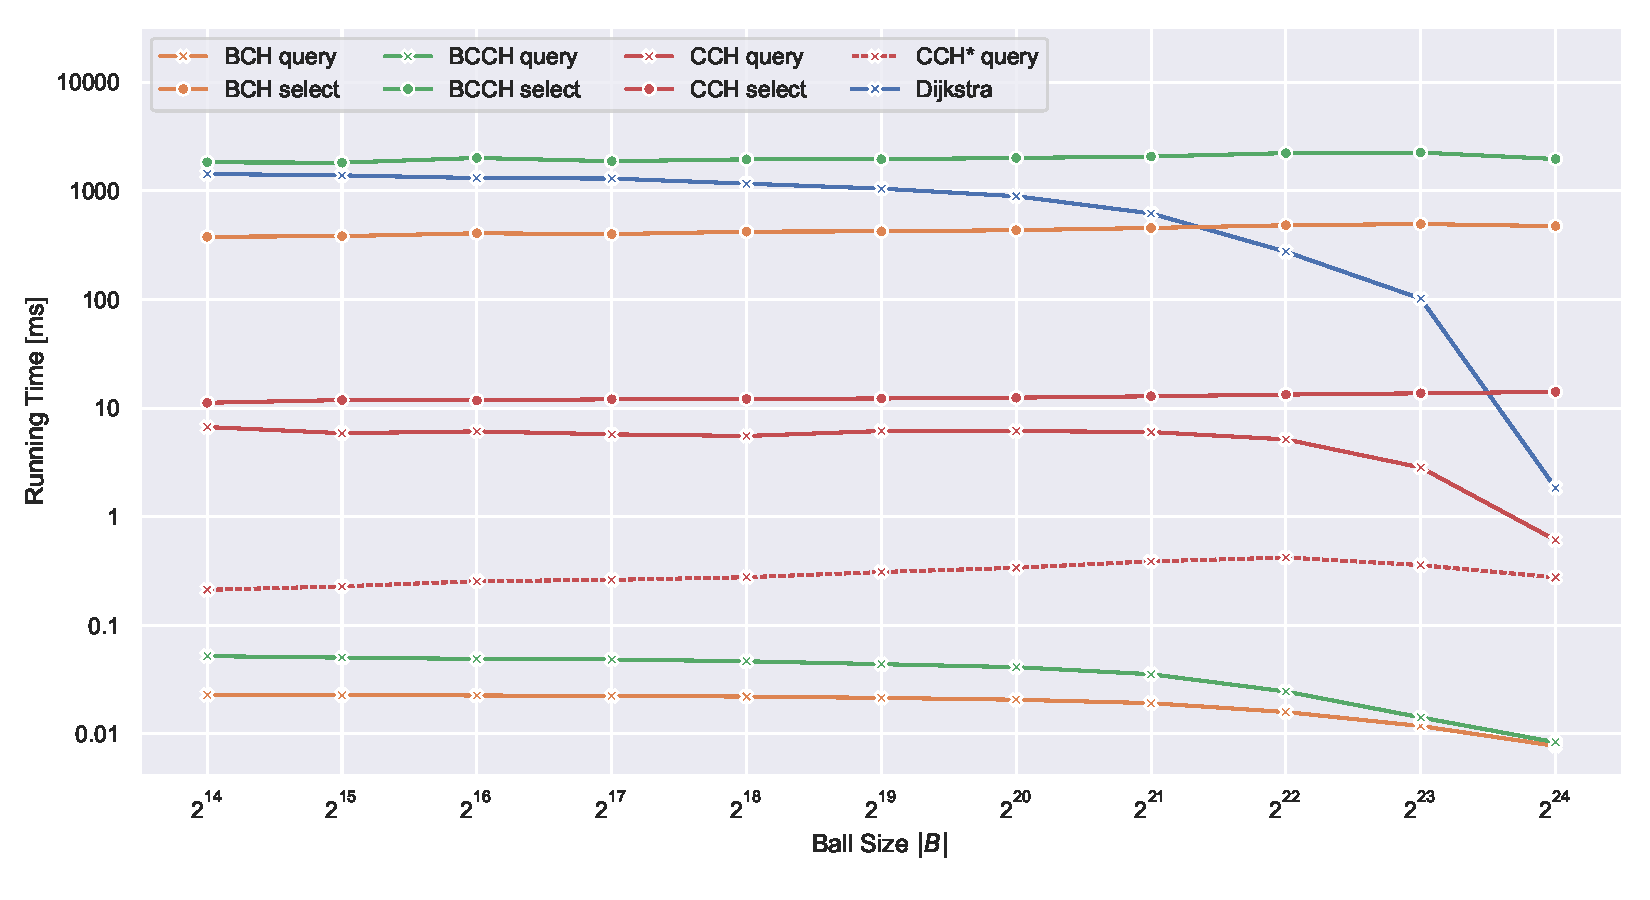
\includegraphics[width=\linewidth]{fig/knn_ball_size.pdf}
% \caption{
% Selection and query times of various closest-POI algorithms with $|P| = 2^{14}$ POIs picked at random from a ball of varying size $|B|$.
% Queries find the $k = 4$ closest POIs.
% }\label{fig:knn_ball_size}
% \end{figure}

% \begin{figure}
% \centering
% 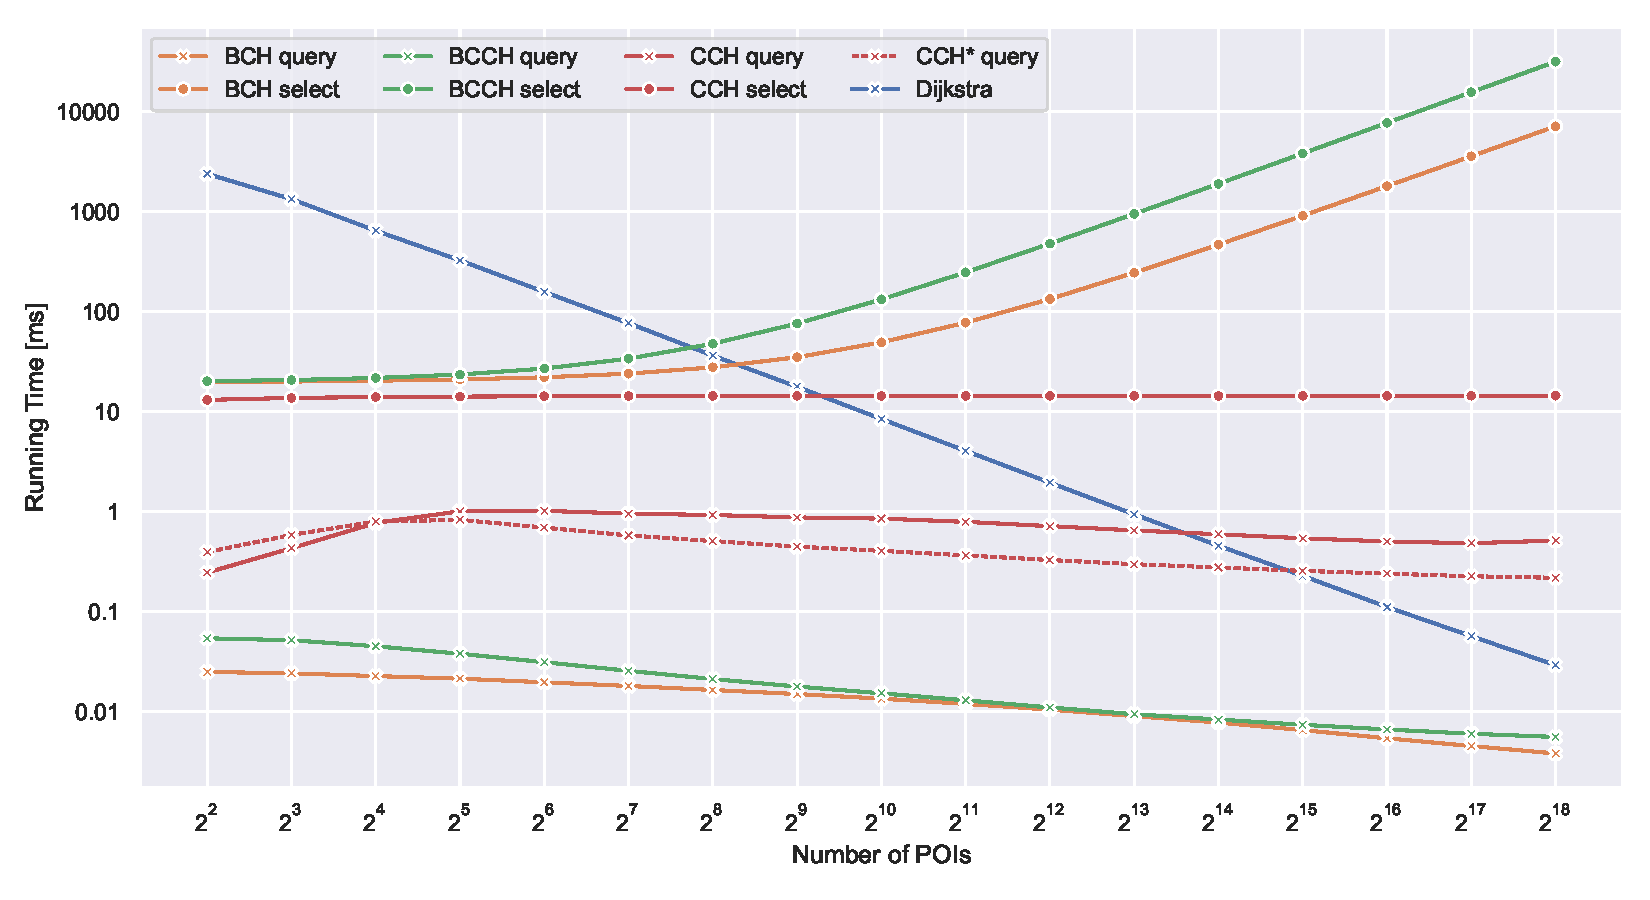
\includegraphics[width=\linewidth]{fig/knn_num_pois.pdf}
% \caption{
% Selection and query times of various closest-POI algorithms with a varying number $|P|$ of POIs picked at random from a ball of size $|B| = |V|$.
% Queries find the $k = 4$ closest POIs.
% }\label{fig:knn_num_pois}
% \end{figure}

% \begin{figure}
% \centering
% 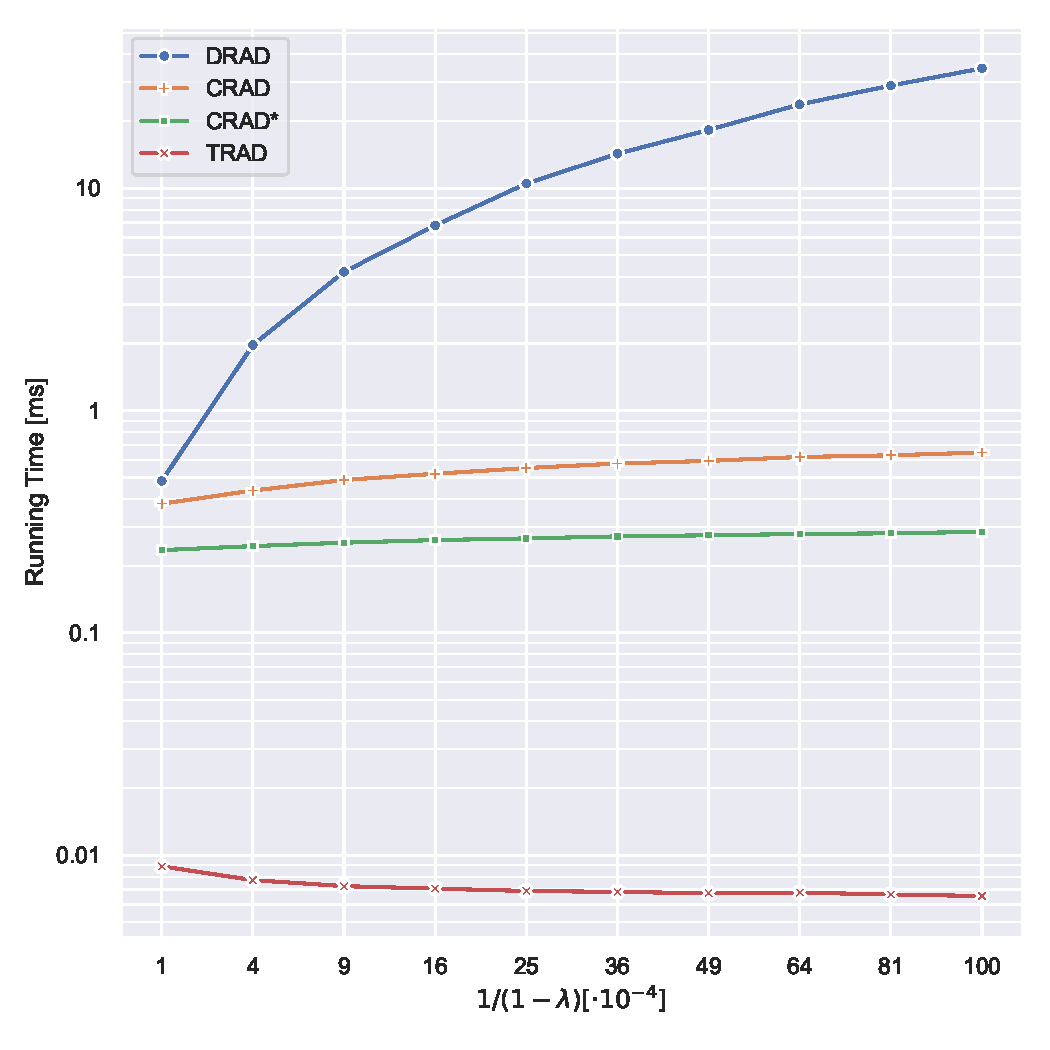
\includegraphics[width=.6363\linewidth]{fig/knn_demands.pdf}
% \caption{
% Time to generate a single trip with different demand generators for various values of $\lambda$.
% }\label{fig:knn_demands}
% \end{figure}

\end{document}
